%\documentclass[11pt,a4paper,openright]{report}
\documentclass[twoside]{template/iitbreport}

%% Default spacing: 1.5
%% Default font size: 12pt
%% Default font: txfonts (similar to times new roman) 

%% Selectively comment out sections that you want to be left out but
%% maintaining the page numbers and other \ref
%\includeonly{%
%  introduction/introduction,
%  lit/literature,
%  expt/experimental,
%  rnd/results, 
%  dec,abs,pub,ack
%}

%%% Some commonly used packages (make sure your LaTeX installation
%%% contains these packages, if not ask your senior to help installing
%%% the packages)

\usepackage{booktabs}
\usepackage{bibentry}
\usepackage{subcaption}
\usepackage{array}
\usepackage{makecell}
\usepackage{comment}
\graphicspath{{chapters/introduction/images/}
              {chapters/modelling/images/}
              {chapters/lincontrol/images/}
              {chapters/hardware/images/}
              {chapters/results/images/}
              {chapters/appendix/images/}
             }

%%% Macro definitions for Commonly used symbols
% \newcommand{\Rey}{\ensuremath{\mathrm{Re}}}
% \newcommand{\avg}[1]{\ensuremath{\overline{#1}}}
% \newcommand{\tenpow}[1]{\ensuremath{\times 10^{#1}}}
% \newcommand{\pder}[2]{\ensuremath{\frac{\partial#1}{\partial#2}}}

% Referencing macros
%\newcommand{\Eqref}[1]{Equation~\eqref{#1}}
%\newcommand{\Tabref}[1]{Table~\ref{#1}}
%\newcommand{\Figref}[1]{Figure~\ref{#1}}
%\newcommand{\Appref}[1]{Appendix~\ref{#1}}


\begin{document}
	
%%********************************Frontmatter***********************
% In frontmatter everything comes with roman numbering	
\pagenumbering{roman}
\setcounter{page}{1}

%*******************************************************************
%                         Title Page                            
%*******************************************************************
%\title{Modelling and Control of WEDM Processes for Cutting of Si-Wafers}
\title{Design and Control of Pulsed Power Supply for WEDM for Fabrication of Silicon Wafers for Photovoltaics}
\author{Akshay Khadse}

%% Print the date. Today's date comes by default, change it here to 
%% other date format, if required:

%\date{\today}
\date{2018}


%% The type of the report can be set here

%\reporttype{A Seminar Report}
%\reporttype{A Thesis}
\reporttype{A Dissertation}
%\reporttype{A Project Report}

%% Name of the degree
%\degree{Doctor of Philosophy}
\degree{Master of Technology}


%% Department/Centre Name
\dept{Department of Electrical Engineering}

%% Supervisor and cosupervisor/excosupervisor are not essential parts
%% of a report title page, as it is your report!

%% But if you **have** to put it uncomment these
\supervisor{Prof. S. V. Kulkarni}
%\cosupervisor{Co-super name}
%\excosupervisor{External Supervisor}

%% Roll number
\rollnum{153079011}

\maketitle

%*******************************************************************
%                         Copyright Page                          
%******************************************************************* 
%\mycopyright                    

%*******************************************************************
%                         Dedication Page                         
%*******************************************************************
%\dedication[Dedicated to \ldots]        
%\addintoc{Dedication}

%*******************************************************************
%                        Certificate Page                         
%*******************************************************************
%\makecertificate[change title name]{report type} 
%\makecertificate{seminar report} 
%\makecertificate{thesis}
%\makecertificate{dissertation}
%\makecertificate{project report}

%\addintoc{Certificate}

%*******************************************************************
%                         Approval Sheet                         
%*******************************************************************
%\makeapproval{thesis}
\makeapproval{dissertation}

%*******************************************************************
%                          Declaration                           
%*******************************************************************
%=============================== declaration.tex ==============================
\begin{Declaration}
\noindent
I declare that this written submission represents my ideas in my own words and where others' ideas or words have been included, I have adequately cited and referenced the original sources. I declare that I have properly and accurately acknowledged all sources used in the production of this report. I also declare that I have adhered to all principles of academic honesty and integrity and have not misrepresented or fabricated or falsified any idea/data/fact/source in my submission. I understand that any violation of the above will be a cause for disciplinary action by the Institute and can also evoke penal action from the sources which have thus not been properly cited or from whom proper permission has not been taken when needed.

\DecSign[\today]

\end{Declaration}
%============================================================================== 
%\addintoc{Declaration}

%******************************************************************
%                          Abstract                             
%******************************************************************  
\begin{Abstract}
%Advancement in photovoltaics as an alternative energy resource is restricted due to the limitations in the manufacturing process of thin silicon wafers. Traditional abrasive methods lead to higher kerf (material) losses. Application of micro-drilling process of Wire Electro Discharge Machining (WEDM) is a viable alternative to such traditional methods. However, WEDM is not as well established for cutting of semiconductors as it is for metals due to the lack of electrical characterisation of metal-dielectric-semiconductor conduction.

Dissemination of photovoltaics is limited due to large payback period and huge capital costs. Cost of raw silicon and that of its fabrication contribute major expenses during initial stages of photovoltaics manufacturing chain. Cost of fabrication of silicon wafers can be reduced by alternative manufacturing processes such as Wire Electric Discharge Machining.

This report summarises the work directed towards the fabrication of an indigenous power supply unit for such unconventional load investigations. The pulsed power supply for this purpose is designed in this work. A parallel converter topology comprising of two modified DC-DC converters is described.

The procedure to derive the linear and nonlinear state space model of this modified converter is presented. Three linear control strategies viz. PID, current mode control, and compensator based control have been tried and the simulation results are included for this converter. The hardware setup employing linear control has been developed for this purpose. The results of initial experimentation are also presented.

The sliding mode control technique is reviewed and a modified version is simulated to verify mitigation of steady state error.
\end{Abstract}
%******************************************************************
%                         Contents list                         
%******************************************************************
\setcounter{tocdepth}{1}
%\figurespagefalse
%\tablespagefalse
\makecontents % Creates toc, lof, and lot

%******************************************************************
%                        Notations                              
%******************************************************************
\notations[4cm]{List of Symbols}      

%%********************************Mainmatter***********************
% In mainmatter everything comes with arabic numbering	
\cleardoublepage
\setcounter{page}{1}
\pagenumbering{arabic}

%******************************************************************
%                         Chapters                           
%****************************************************************** 
\Chapter{Introduction}
\label{chap:introduction}
	Solar energy is a prominent source of renewable energy across the globe. India has aimed to reach for 100 GW contribution from solar installations alone till 2022 \cite{mnreReport}. Silicon is the most preferred material for manufacturing the photovoltaic (PV) panels. This manufacturing process is energy intensive and thereby very costly. Extracting ingots from raw silicon accounts for 20\% of the total energy consumption throughout the process \cite{del09}. Hence, the initial cost of solar installation is higher. This can be reduced by finding better options for manufacturing silicon wafers.

\section{Methods for dicing silicon}
	The two popular methods for cutting of silicon are i) Wire loose slurry method and ii) Diamond saw cutting method. These methods, being abrasive in nature, lead to micro-fractures and cracks as deep as 20 $\mu$m in the final product. Because of this, the wafer size gets limited to 180 $\mu$m \cite{sopori13}. Also, about 50\% of the ingot material is lost as kerf losses \cite{joshi10}. These methods have other disadvantages like contamination of wafers due to slurry, etc. \cite{moeller2015}.

\subsection{Wire Loose Slurry Method}
	In this method, the workpiece is secured and a moving wire is used for cutting. The entire assembly is immersed in abrasive slurry to improve the cutting rate. The principle of operation of this technique is similar to that of a saw. The only difference is that slurry is used as abrasive material. This method is preferred for its improved processing time when multiple parallel wires are used on single ingot.

\subsection{Diamond Saw Cutting}
	A diamond coated abrasive wire is used in this method as opposed to the non abrasive wire from the previous method. This method can be used without any immersing medium. However, the assembly is usually immersed in water as diamond saw blades have been found to work better in wet conditions. Similar to the above method, multiple parallel abrasive wires are used in practice to improve the throughput of this process.

\subsection{Wire Electric Discharge Machining}
	WEDM is a novel machining process in which a moving thin wire electrode is used. Copper, tungsten, or brass wires with diameters of the order $10^{-4}$ m are commercially preferred. A small gap is always maintained between the work-piece and the wire. It is a through hole machining method capable to machine high strength and temperature resistance materials. Figure \ref{fig:lit-1} depicts the apparatus used for the experimentation hinted earlier, which schematically shows the arrangement in the actual WEDM machine.

	\begin{figure}[H]
		\centering
		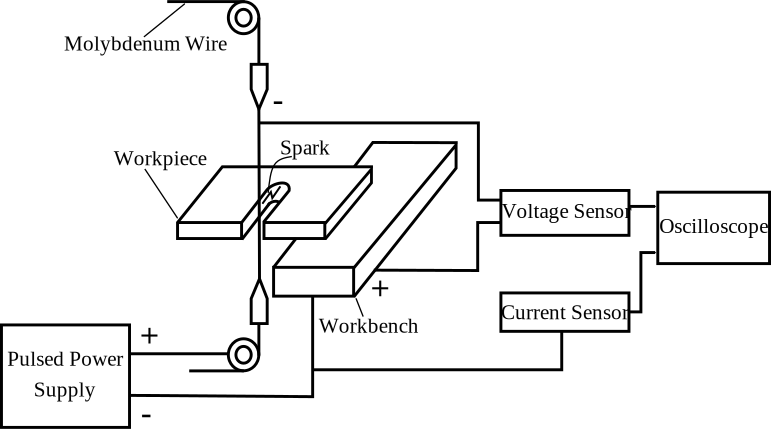
\includegraphics[width=0.8\textwidth]{wedm-diag}
		\caption{Diagrammatic representation of WEDM}
		\label{fig:lit-1}
	\end{figure}

	In WEDM, erosion of the workpiece material achieved by repetitive sparking in the gap between the work-piece and wire. Electrical energy from a pulsating DC power supply operating in the frequency range 0.5 to 30 kHz is used to generate the ionisation potential between the cathode and the anode at temperatures ranging from 8000$^\circ$ to 12000$^\circ$. Once turned off, plasma channel implodes, molten particles are flushed away and the gap recovers its dielectric strength. WEDM uses a fine wire travelling through the work-piece at a constant rate to avoid wire breakage due to formation of localised hotspots.

	%In the final product, a taper \cite{ho2004state} ranging from 15$^\circ$ for 100 mm thick to 30$^\circ$ for a 400 mm thick work-piece can be achieved. Typical Cutting Rates (CR) are 30 mm/min for 50 mm thick D2 tool steel and 750 mm/min for 150 mm thick aluminium.
	
	WEDM is a non contact micro-drilling process which can be used to cut free form contours from large solid metal workpieces. Experiments have shown that kerf width can be reduced from 250 $\mu$m in abrasive saw cutting to 50 $\mu$m in WEDM resulting in net material saving of 200 - 300\% \cite{dongre2015multi}. This method presents a promising alternative for application to silicon wafer manufacturing. Hence, the long term goal of this project is to optimise the manufacturing process of silicon wafers.

\section{Motivation}
	Although this process has been demonstrated for cutting of semiconductors and even ceramics \cite{sanchez2001development}, it is not as well established for these non conventional materials as it is for the metals. One reason for this is the lack of electrical characterisation of metal-semiconductor-dielectric sparks. The experimentation done to investigate this has so far led to the conclusion that the spark gap VI characteristics of silicon are very different from that of the steel \cite{kane2017aps}. Hence, it is important to find a reliable model for spark gap in this setting. However, the commercially available EDM machines are optimised for metals and have only discrete setting ranges. This has been acknowledged by \citet{levy1990wed}.

	Hence, the available machines are inadequate to carry out further experimentation as they provide discretely spaced setting ranges. An indigenously designed power supply along with a test setup is therefore required to carry out load investigations and optimise the process of Si-ingot cutting for PV applications.

\section{Scope}

	The goal of this project is to develop a pulsed power supply unit for WEDM which could deliver a variable ignition voltage and regulate the spark gap current. Such a regulated power supply is required for the experimentally understanding the WEDM process for silicon. The scope of this project extends to:
	\begin{itemize}
	\item Research of the existing pulsed power supplies is done to determine a suitable converter topology.
	\item Linear and  nonlinear modelling of the proposed supply.
	\item Controller design and verification via simulation for:\\
	1) Linear controllers: PI controller, current mode control, and compensator based control\\
	2) Nonlinear controller: Sliding mode control
	\item Design and fabrication of current and voltage sensing boards.
	\item Assembling the power circuit components with the digital signal processor.
	\item Implementing and hardware testing the PI controller.
	\end{itemize}

\section{Organisation of report}
	This report summarises the work done in design, modelling, and control of prototype power supply for Si-Ingot cutting by WEDM. Chapter \ref{chap:introduction} and \ref{chap:litreview} are dedicated to the introduction and the literature available on this regard.
	
	Chapter \ref{chap:modelling} describes the modelling process followed for deriving the dynamical models of the proposed power supply. In depth explanation of the time averaging technique of linear modelling and the direct technique for nonlinear modelling is provided here. The changes in system dynamics due to the deviation from the standard converter topology are also highlighted via the bode plots.

	The controller design of the aforementioned power supply is discussed in chapter \ref{chap:lincontrol}. The design procedures of linear controllers viz. PI controller, peak current mode control, and compensator based control form the first part of this chapter. This is followed by the theory and design of sliding mode controller.
	
	Chapter \ref{chap:hardware} is a detailed account of the hardware implementation of the pulsed power supply. This chapter describes the procedure followed for the selection of the passive components for the converter. The designs of sensor and interfacing boards, and the power circuit are described here.
	
	The simulation and the hardware experimentation results are included in the chapter \ref{chap:results}. This includes the simulation observations for the linear controllers and the hardware experimentation results with the PI controller. The current source time response is analysed in depth to reason out the observed behaviour. Towards the end of this chapter are the conclusions and the some possible future avenues that can be pursued.
	
	

\Chapter{Literature Review}
\label{chap:litreview}
	WEDM is a complex cutting process. The spark this process exhibits stochastic behaviour. There are many parameters like discharge frequency, discharge current, wire feed rate etc which affect the cutting performance of WEDM. Besides pulsed DC power supply, research avenues in other areas of WEDM are also explored. Following subsections give a brief account of the literature looked at in this regard.

%	WEDM is an extensive process with a large number of parameters like pulse duration, discharge frequency, discharge current, wire feed rate, etc., which in turn affect the output product in terms of surface roughness, cutting rates and material removal rates (MRR), etc. While a lot of literature is available for steel and other metals ranging from effects of process parameters on cutting to improve the MRR, CR and surface finish, this chapter presents the relevant material available on process modelling, monitoring and control.

\section{WEDM Control}
\subsection{Process Modelling}
	A influence of the work-piece material and pulse parameters is modelled by \citet{spur1993anode} in 1993. The spark-gap discharge has been studied and simulated by \citet{han2002high}. They have also developed an adaptive control system for maintaining near ideal machining parameters.

\subsection{Fuzzy Control Systems}
	Fuzzy control systems have been a popular choice in this application because of independence from the requirement of comprehensive mathematical models. \citet{kinoshita1976study} modelled the effects of various mechanical and electrical parameters in the WEDM. \cite{de1982has} analysed the spark ignition delay and developed a pulse classifier based on this. They also determined how various machining parameters are affected by this delay.

\subsection{Wire Breakage Avoidance}
	\citet{kinoshita1982control} correlated the frequency of the EDM pulses to the breakage of wire electrode. An observer has also been developed that controls the pulse generator and wire translation to avoid wire breakage. The increase in localised temperature due at certain points of wire has been found to cause its breakage. To prevent this, a monitoring and control system has been developed in \cite{kunieda1990line}.

\subsection{Wire Lag and Wire Vibrations}
	\citet{dauw1994high} used an optical sensor for on-line monitoring the wire position and a controller for high speed. It has also been proposed to increase the gap distance to prevent wire gauging and breakage on high curvature areas of the work-piece \cite{wang2003computer} and many contour planning systems for WEDM apply this today. The transient behaviour of the wire vibrations are described in \cite{mohri1998system} and some mathematical models have been developed.

\subsection{Adaptive Control Systems}
	Much of the work uses adaptive control systems in this field for maintenance scheduling, machining variable height workpieces and predicting the thermal overload. Workpieces with non-uniform thickness have been found to exhibit increased thermal density during machining \cite{kinoshita1982control}. An estimator has been designed to determine the workpiece height and regulate the machining frequency accordingly in \citet{rajurkar1997wedm}.
	
\section{Pulsed Power Supplies}
	Very few research papers are available as far as WEDM power supplies are concerned. Most of the information is either proprietary or lies in patents. \citet{sen2003developments} have briefed about the WEDM power supplies developed till 2003. A few other authors have given newer topologies for WEDM power supplies.
\subsection{Basic Relaxation Circuit Based Power Supplies}
	A RC relaxation circuit with the spark gap connected across the spark gap can cause the breakdown of the dielectric medium. Spark gets initiated when the capacitor connected in parallel to the load is charged to the breakdown voltage of the gap. Due to this, the capacitor is discharged and starts charging again from the supply. The resistance is required to prevent the formation of a continuous arc in the gap. A slightly modified version of this circuit employs a freewheeling diode to restrict the reversal of the current flow direction.

	In another power supply, a tube triode pulser or DC interrupter is used to generate high frequency pulses which are fed to the spark gap. These supplies have the advantage of low energy consumption and higher frequency operation over the RC relaxation power supplies.
\subsection{Switching Circuit Power Supplies}
	The operation of transistor as a switch is exploited to control the current from the DC supply to the spark gap. These supplies provide control over the spark current if multiple transistors are used in series and parallel configuration.

	Thyristorised power supplies along with a RLCL oscillator circuit for charging and discharging of the capacitor across the spark gap are also possible. In this, a thyristor and a diode is used to control the duty of machining based on a low voltage pulsed generator. These type of supplies need forced commutation.
\subsection{LCC Resonant Converter}
	A LCC resonant converter tuned to its natural frequency is used along with a half wave rectifier to generate high ionisation voltages across the spark gap. An improved version of this power supply has inherent short circuit protection.\cite{sen2003developments}

	\citet{casanueva2008new} have proposed a bipolar supply to minimise the corrosion due to the electrolysis effect of the unipolar supplies. This power supply uses a full bridge rectifier to control the current fed to a LC series parallel resonant circuit. Finally, a transformer in the output stage is used to generate high ionisation voltages across the gap.

\subsection{Parallel Converters Based Power Supplies}
	A EDM power supply based on a current controlled buck converter and a rectifier is proposed by \citet{looser2010novel}. The rectifier is used to generate the voltage required for the breakdown of the spark gap while the buck converter controls the amount of current through the spark gap. These power supplies can be used for dry EDM with large gap lengths.
	
	A similar power supply is developed by \citet{tastekin2009novel}. The ignition voltage is built up by means of a voltage controlled two quadrant DC-DC converter instead of a rectifier while the current is controlled by a buck converter. This allows for independent control of spark gap voltage and current. This topology has been further developed in this project.
\Chapter{Power Supply Design and Modelling}
\label{chap:modelling}
Power supply for the WEDM process delivers intermittent current and voltages across the electrode-dielectric-silicon ingot assembly. The pulsed nature of this power supply makes the design for such circuit difficult. This chapter describes the working of an ideal power source for the WEDM process followed by its converter topology. The linear and nonlinear models are then derived for this converter.

\section{Working Principle}
	Figure \ref{fig:working-1} represents the functional configuration of a pulsed power supply in which an ideal current source $I_o$ and ideal voltage source $V_o$ are connected in parallel across the spark gap load $E$. The current and voltage waveforms across the load are shown in figure \ref{fig:working-2}
	\begin{figure}[H]
		\begin{subfigure}{0.49\textwidth}
			\vspace{0.5cm}
			\centering
			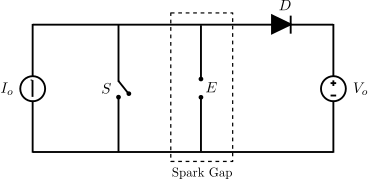
\includegraphics[width=\linewidth]{rep-diag-master}
			\caption{Representative diagram}
			\label{fig:working-1}
		\end{subfigure}
		\begin{subfigure}{0.49\textwidth}
			\centering
			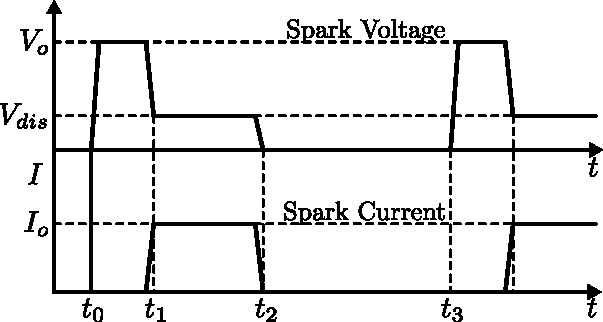
\includegraphics[width=\linewidth]{working-wf-master}
			\caption{Load voltage and current}
			\label{fig:working-2}
		\end{subfigure}
		\caption{Working of WEDM supply}
	\end{figure}

\subsection{Pre-Breakdown}
	During times $t=t_0$ and $t=t_1$, the current source causes the diode $D$ to turn on and $I_o$ flows through $D$ to the ideal voltage source $V_o$. The voltage across the load terminals is $V_o$ because $D$ remains in a conduction state from $t_0$ to $t_1$. This application of voltage across the spark gap terminals causes the gap to break down at $t=t_1$. This breakdown delay time depends on the dielectric strength and the magnitude of the applied voltage.
	\begin{figure}[H]
		\centering
		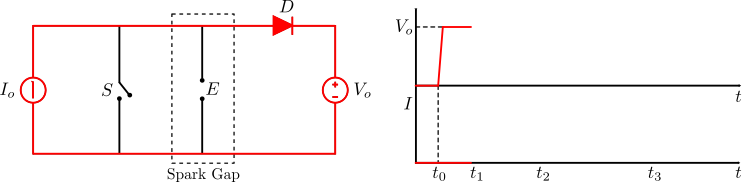
\includegraphics[width=\textwidth]{working-1}
		\caption{Pre-breakdown stage}
		\label{fig:working-1}
	\end{figure}

\subsection{Sparking}
	Due to breakdown of dielectric, current $I_o$ starts flowing through the spark gap $E$ and the diode $D$ turns off. If the spark gap is modelled as a resistance, the voltage across terminals is $V_{dis}$ and is equal to $I_or_{gap}$. The silicon ingot now erodes along the length of moving wire electrode.
	\begin{figure}[H]
		\centering
		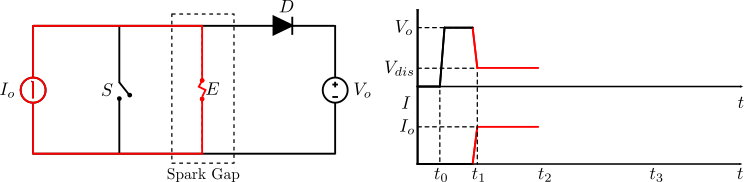
\includegraphics[width=\textwidth]{working-2}
		\caption{Sparking stage}
		\label{fig:working-2}
	\end{figure}	

\subsection{Dead Time}
	The \emph{dead} time zone serves three purposes: (a) avoids a sustained arc (and hence a short circuit) (b) gives time for removal of debris from the gap and (c) allows the tool electrode to move closer to the workpiece. This is achieved closing the switch $S$ at time $t=t_2$. When $S$ is closed, the current $I_o$ flows through current source and switch and dielectric strength of the medium is recovered by flushing fresh dielectric over the gap.
	\begin{figure}[H]
		\centering
		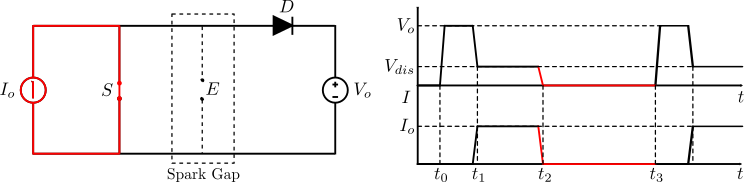
\includegraphics[width=\textwidth]{working-3}
		\caption{Dead time stage}
		\label{fig:working-3}
	\end{figure}
	When the gap is fully recovered, a new machining cycle is started at time $t=t_3$ by opening the switch $S$. The erosion takes place for about 10\% of the entire machining period. Thus, the power is supplied to load only for this fraction of the machining period.

\section{Converter Topology}
	\begin{figure}[h]
		\centering
		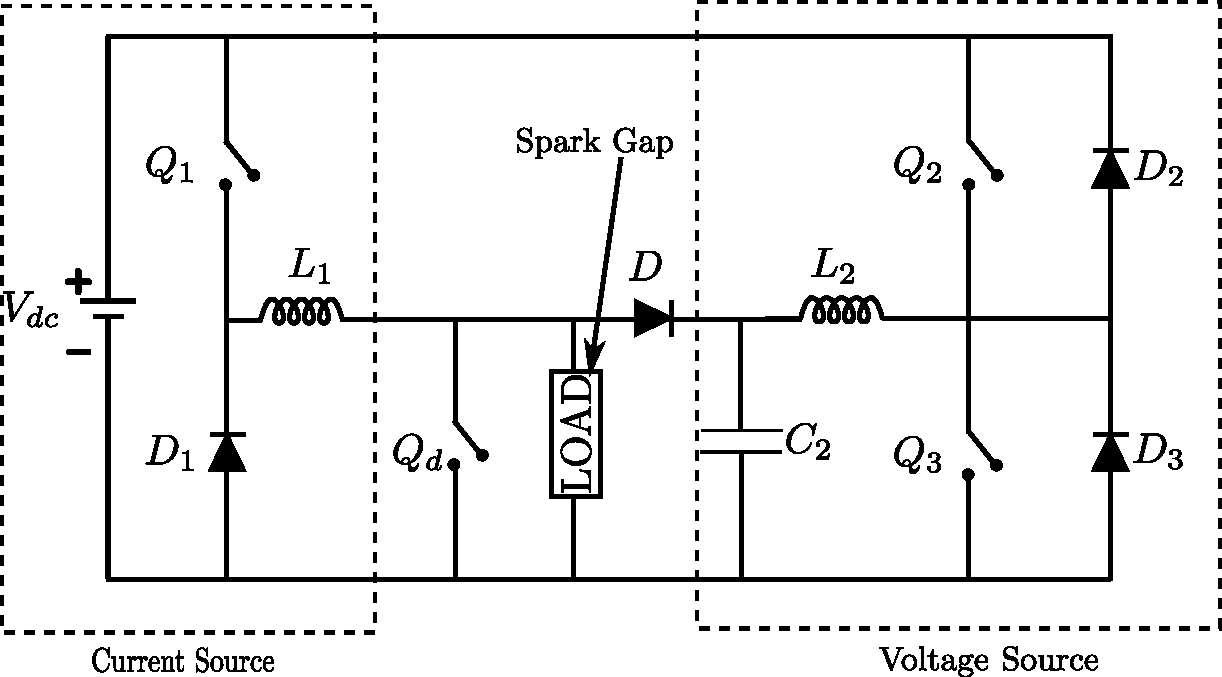
\includegraphics[width=0.9\textwidth]{conv-top-master}
		\caption{Converter topology for WEDM power supply}
		\label{fig:working-3}
	\end{figure}
	This section describes the practical implementation of the ideal current and voltage sources depicted in figure \ref{fig:working-1}. One realisation of such power supply is proposed by Tastekin et al. in \cite{tastekin2009novel} in which a single quadrant and a two quadrant DC-DC converter is connected to the same DC link. A single quadrant converter is used as current source by controlling the inductor current and removing the filter capacitance. The voltage source is realised by controlling the output voltage of the two quadrant converter. Figure \ref{fig:working-3} depicts this configuration using high frequency power electronic switches.

	Constant voltage of $V_o$ is maintained at the load terminals of the two quadrant converter. However, when switch $S$ in figure \ref{fig:working-1} is opened, the current $I_o$ goes through $D$ to the capacitor of the two quadrant converter. This acts as a disturbance to the voltage source controller and must be rejected at the earliest to maintain the constant voltage across the load terminals.

	This implementation does not use transistors and resistors, hence the only losses incurred are the switching and conduction losses of the power electronic switches, and the inductor copper losses.
	
\section{Linear Modelling}
	%The power supply depicted in figure \ref{fig:working-3} is composed of three components viz. single quadrant converter acting as current source, two quadrant converter acting as voltage source, and the ignition switch. 
	A controller is required to regulate the current of the quadrant converter and the voltage of the the two quadrant converters each, hence the state space model for these converters is found out. This section explains the time averaging method to arrive at the small signal models between the output voltage or current and the duty ratio of the switches for both the converters.

\subsection{Voltage Source}
	\begin{figure}[H]
		\begin{subfigure}{0.49\textwidth}
			\centering
			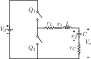
\includegraphics[width=\linewidth]{2quad-mod-master}
			\caption{Modified}
			\label{fig:working-4}
		\end{subfigure}
		\begin{subfigure}{0.49\textwidth}
			\centering
			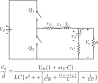
\includegraphics[width=\linewidth]{2quad_norm}
			\caption{Standard}
			\label{fig:working-4b}
		\end{subfigure}
		\caption{Simplified circuit of two quadrant converter}
		\label{fig:2quad-comparison}
	\end{figure}
	Figure \ref{fig:working-4} represents the simplified circuit for the two quadrant converter which is to be, hence the small signal transfer function $\dfrac{\hat{v}_o}{\hat{d}}$ is to be found out. The current through the inductor $L$ and the voltage across capacitor $C$ are considered as the state variables.

	When the switch $Q_2$ is on i.e. for time $DT_s$, current flows though $V_d$, $Q_2$, $r_{L}$, $L$, $r_{C}$ and $C$. Applying Kirchhoff's Voltage Law along this path gives
	\begin{equation}
		V_d - L \dot{x}_1 - r_{L}x_1 - r_{C}x_1-x_2 = 0
		\label{eq:mod1}
	\end{equation}
	From current through the inductor and the capacitor is same, therefore
	\begin{equation}
		x_1 = C\dot{x_2} 
		\label{eq:mod2}
	\end{equation}
	The output voltage is
	\begin{equation}
		V_o = r_{C}x_1 + x_2
		\label{eq:mod3}
	\end{equation}
	\begin{equation}
		\begin{split}
		\therefore \dot{x}_1 &= -\dfrac{r_{L}+r_{C}}{L}x_1 -\dfrac{1}{L}x_2+\dfrac{1}{L}V_d\\
		\dot{x}_2 &= \dfrac{1}{C}x_1\\
		V_o &= r_{C}x_1 + x_2
		\end{split}
		\label{eq:mod4}
	\end{equation}
	When $Q_2$ is off i.e. for time $(1-D)T_s$, current flows through  $D_3$, $r_{L}$, $L$, $r_{C}$ and $C$. Applying Kirchhoff's Voltage Law along this path gives
	\begin{equation}
		- L \dot{x}_1 - r_{L}x_1 - r_{C}x_1-x_2 = 0
		\label{eq:mod5}
	\end{equation}
	Also,
	\begin{equation}
		x_1 = C\dot{x_2} 
		\label{eq:mod6}
	\end{equation}
	The output voltage is
	\begin{equation}
		V_o = r_{C}x_1 + x_2
		\label{eq:mod7}
	\end{equation}
	\begin{equation}
		\begin{split}
			\therefore \dot{x}_1 &= -\dfrac{r_{L}+r_{C}}{L}x_1 -\dfrac{1}{L}x_2\\
			\dot{x}_2 &= \dfrac{1}{C}x_1\\
			V_o &= r_{C}x_1 + x_1
		\end{split}
		\label{eq:mod8}
	\end{equation}
	Constructing the state vector $x$ as
	\begin{equation}
		x =
		\begin{bmatrix}
			x_1\\x_2
		\end{bmatrix}
		\label{eq:mod9}
	\end{equation}
	In equation \eqref{eq:4}, let
	\begin{equation}
		A_1=
		\begin{bmatrix}
			-\dfrac{r_{L}+r_{C}}{L} & -\dfrac{1}{L}\vspace*{2mm}\\
			\dfrac{1}{C} & 0
		\end{bmatrix}
		\quad
		B_1=
		\begin{bmatrix}
			\dfrac{1}{L} \vspace*{2mm}\\ 0
		\end{bmatrix}
		\quad
		C_1 =
		\begin{bmatrix}
			r_{C} & 1
		\end{bmatrix}
		\label{eq:mod10}
	\end{equation}
	\begin{equation}
		\begin{split}
			\therefore \dot{x} &= A_1 x + B_1 V_d\\
			V_o &= C_1 x
		\end{split}
		\label{eq:mod11}
	\end{equation}
	In equation \eqref{eq:5}, let
	\begin{equation}
		A_2=
		\begin{bmatrix}
			-\dfrac{r_{L}+r_{C}}{L} & -\dfrac{1}{L}\vspace*{2mm}\\
			\dfrac{1}{C} & 0
		\end{bmatrix}
		\quad
		B_2=
		\begin{bmatrix}
			0 \vspace*{2mm}\\ 0
		\end{bmatrix}
		\quad
		C_1 =
		\begin{bmatrix}
			r_{C} & 1
		\end{bmatrix}
		\label{eq:mod12}
	\end{equation}
	\begin{equation}
		\begin{split}
			\therefore \dot{x} &= A_1 x + B_1 V_d\\
			V_o &= C_1 x
		\end{split}
		\label{eq:mod13}
	\end{equation}
	Equation \eqref{eq:mod11} is valid for $dT_s$ and equation \eqref{eq:mod13} is valid for $(1-d)T_s$. Time averaging equations \eqref{eq:mod11} and \eqref{eq:mod13} leads to
	\begin{equation}
	    \begin{split}
    		\dot{x} &= [dA_1+(1-d)A_2]x + [dB_1 + (1-d)B_2]V_d\\
	    	V_o &= [dC_1+(1-d)C_2]x
		    \label{eq:mod14}
	    \end{split}
	\end{equation}

	Small signal transfer function for this representation is derived by introducing small perturbations in $x$, $V_o$, and $d$ and eliminating the steady state quantities. Complete mathematical treatment is described in pp.324-325 of \citet{book:768263}. The small signal transfer function of the output voltage of two quadrant converter with respect to the duty ratio of the switch $Q_2$ turns out to be \cite{book:768263}
	\begin{equation}
		\therefore \dfrac{\hat{v}_o(s)}{\hat{d}(s)} = C[sI-A]^{-1}[(A_1-A_2)X+(B_1-B_2)V_d]+(C_1-C_2)X
		\label{eq:mod27a}
	\end{equation}
	The scalar form of this transfer function is shown in table \ref{tab:vstf}.
	\begin{table}[h]
	\centering
	\begin{tabular}{|p{6cm}|p{8cm}|} \hline
	\multicolumn{1}{|c|}{Modified} & \multicolumn{1}{c|}{Standard} \\ \hline
	\vspace{-2mm} \(\displaystyle \dfrac{\hat{v}_o(s)}{\hat{d}(s)} = \dfrac{V_{dc}(Cr_Cs+1)}{LCs^2+(Cr_C+Cr_L)s+1} \) & \vspace{-2mm} \(\displaystyle \dfrac{\hat{v}_o(s)}{\hat{d}(s)} = \dfrac{V_{dc}(Cr_Cs+1)}{LC\{s^2+s\left[\dfrac{1}{RC} + \dfrac{(r_C + r_L)}{L} \right]+\dfrac{1}{LC}\}}\) \vspace{1mm} \\ \hline
	\end{tabular}
	\caption{Scalar transfer function of voltage source}
	\label{tab:vstf}
	\end{table}
	
	The bode plot for this transfer function when the values of inductors and capacitors are chosen as described in chapter \ref{chap:hardware} is shown in figure \ref{fig:uncomp-vs}
	\begin{comment}
		\begin{figure}[h]
			\centering
			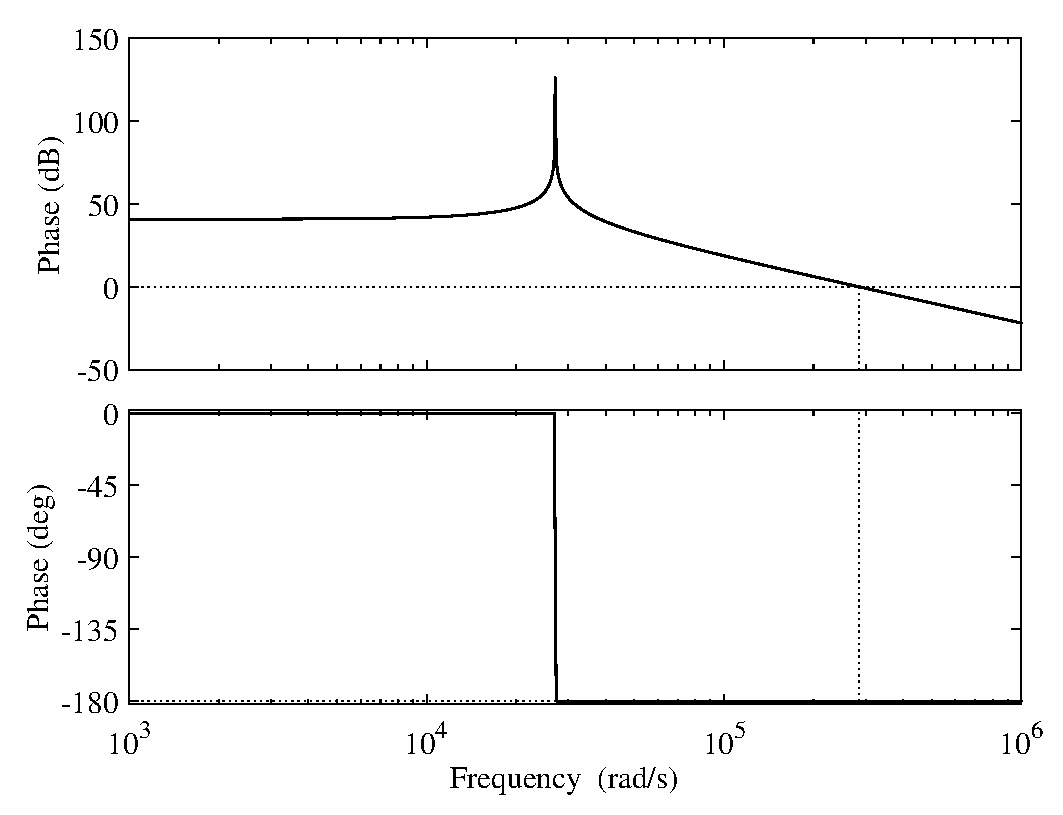
\includegraphics[width=0.8\textwidth]{uncompensated-vs}
			\caption{Bode plot of uncompensated transfer function of voltage source; Gm = $\infty$,  Pm = 0.0166$^\circ$ (at 2.85e+05 rad/s)}
			\label{fig:uncomp-vs}
		\end{figure}
	\end{comment}
	\begin{figure}[H]
		\centering
		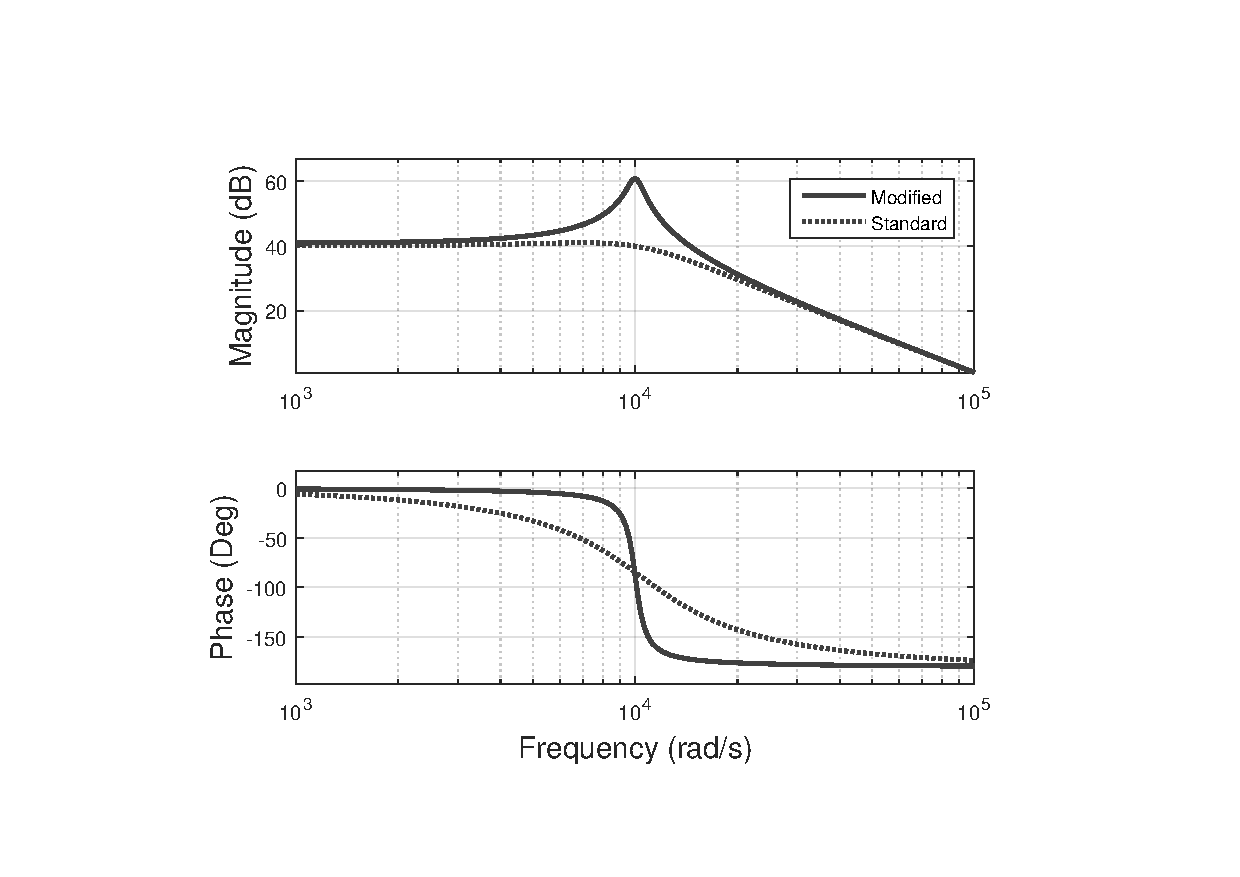
\includegraphics[width=0.7\textwidth]{vs_comparison}
		\caption{Bode plot of voltage source}
		\label{fig:uncomp-vs}
	\end{figure}
	The magnitude of peak in the bode plot of the modified two quadrant converter is more as compared to that of the standard counterpart. The removal of the resistance from the output of the standard two quadrant converter causes reduction in the damping factor which is observable in figure \ref{fig:uncomp-vs}.

\subsection{Current Source}
	\begin{figure}[H]
		\begin{subfigure}{0.49\textwidth}
			\centering
			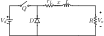
\includegraphics[width=\linewidth]{buck-mod-master}
			\caption{Modified}
			\label{fig:working-5}
		\end{subfigure}
		\begin{subfigure}{0.49\textwidth}
			\centering
			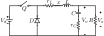
\includegraphics[width=\linewidth]{buck_norm}
			\caption{Standard}
			\label{fig:working-5b}
		\end{subfigure}
		\caption{Simplified circuit of single quadrant converter}
		\label{fig:buck-comparison}
	\end{figure}
	Similar approach is applied for finding out the transfer function of the output current with respect or the duty cycle of the switch $Q_1$ for the single quadrant converter. Figure \ref{fig:working-5} shows the simplified circuit diagram for the same. The current through the inductor $L$ is the only state variable in this case.

	When the switch $Q_1$ is on i.e. for time $dT_s$, current flows though $V_d$, $Q_1$, $r_{L}$, $L$ and $R_L$. Applying Kirchhoff's Voltage Law along this path gives
	\begin{equation}
		V_d - L \dot{x} - r_{L}x - R_Lx = 0
		\label{eq:mod28}
	\end{equation}
		The output current is
	\begin{equation}
		I_o = x
		\label{eq:mod29}
	\end{equation}
	\begin{equation}
		\begin{split}
			\therefore \dot{x} &= -\dfrac{r_{L}+R_L}{L}x +\dfrac{1}{L}V_d\\
			I_o &= x	
		\end{split}
		\label{eq:mod30}
	\end{equation}
	When $Q_1$ is off i.e. for time $(1-d)T_s$, current flows through  $D_1$, $r_{L}$, $L$ and $R_L$. Applying Kirchhoff's Voltage Law along this path gives
	\begin{equation}
		- L \dot{x} - r_{L}x - R_Lx = 0
		\label{eq:mod31}
	\end{equation}
	The output current is
	\begin{equation}
		I_o = x
		\label{eq:mod32}
	\end{equation}
	\begin{equation}
		\begin{split}
			\therefore \dot{x} &= -\dfrac{r_{L}+R_L}{L}x\\
			I_o &= x
		\end{split}
		\label{eq:mod33}
	\end{equation}
	\begin{equation}
		\begin{split}
			\therefore A_1 &= -\dfrac{r_{L}+R_L}{L} = A_2\\
			B_1 &= \dfrac{1}{L} \quad B_2 = 0\\
			C_1 &= 1 = C_2
		\end{split}
		\label{eq:mod34}
	\end{equation}
	The transfer function $\dfrac{\hat{i}_o}{\hat{d}}$ is obtained using equations \eqref{eq:mod34} in following \cite{book:768263} 
	\begin{equation}
		\dfrac{\hat{i}_o(s)}{\hat{d}(s)} = C[sI-A]^{-1}[(A_1-A_2)X+(B_1-B_2)V_d]+(C_1-C_2)X
		\label{eq:mod35}
	\end{equation}
	where
	\begin{align}
		A &= A_1d+A_2(1-d)
		\label{eq:mod36}
	\end{align}
		The scalar form of this transfer function is shown in table \ref{tab:cstf}.
	\begin{table}[h]
	\centering
	\begin{tabular}{|p{4cm}|p{8cm}|} \hline
	\multicolumn{1}{|c|}{Modified} & \multicolumn{1}{c|}{Standard} \\ \hline
	\vspace{-2mm} \(\displaystyle \dfrac{\hat{i}_o(s)}{\hat{d}(s)} = \dfrac{V_{dc}}{(R+r_L)+Ls} \) & \vspace{-2mm} \(\displaystyle \dfrac{\hat{i}_o(s)}{\hat{d}(s)} = \dfrac{V_{dc}(Cr_Cs+1)}{RLC\{s^2+s\left[\dfrac{1}{RC} + \dfrac{(r_C + r_L)}{L} \right]+\dfrac{1}{LC}\}}\) \vspace{1mm} \\ \hline
	\end{tabular}
	\caption{Scalar transfer function of current source}
	\label{tab:cstf}
	\end{table}

	The bode plot for this transfer function when the values of inductors and capacitors are chosen as described in \ref{chap:hardware} is shown in figure \ref{fig:uncomp-cs}
	\begin{comment}
		\begin{figure}[H]
			\centering
			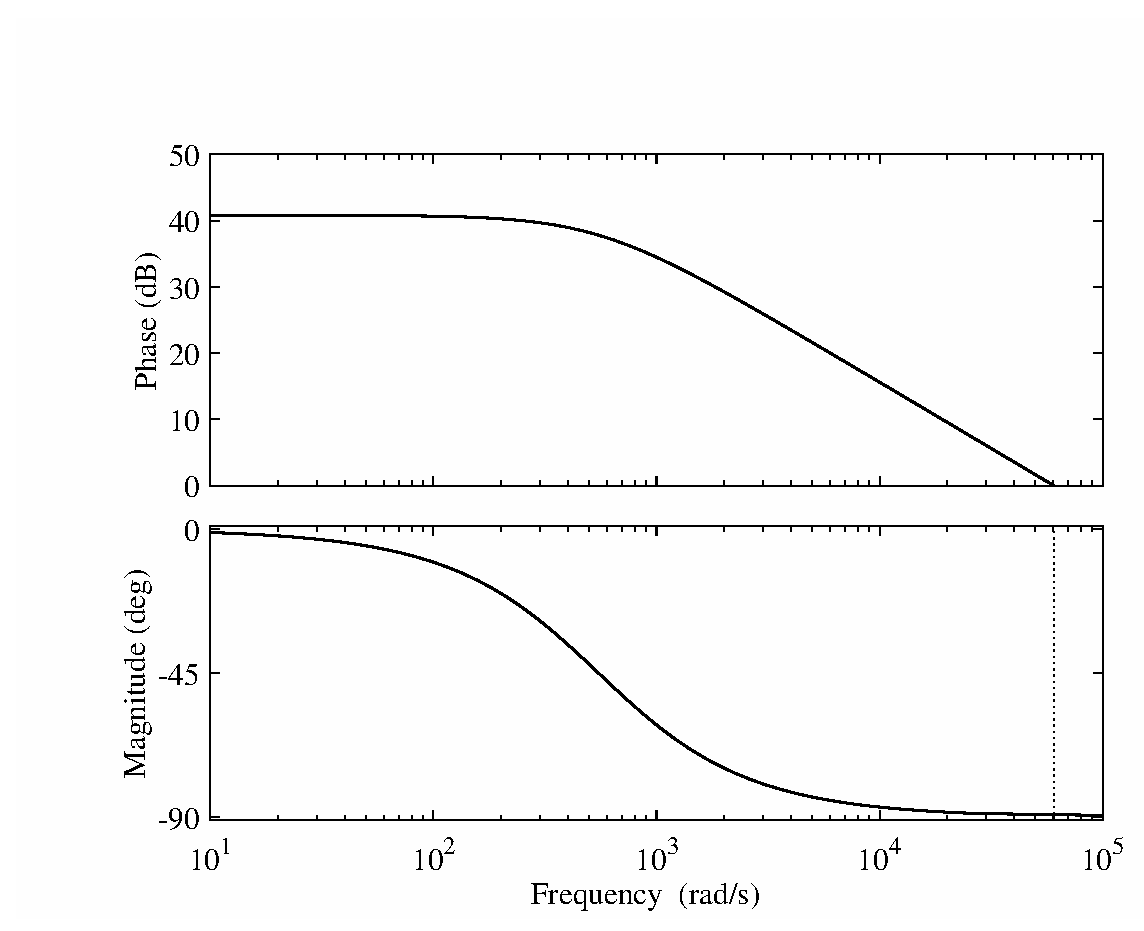
\includegraphics[width=0.8\textwidth]{uncompensated-cs}
			\caption{Bode plot of uncompensated current source transfer function; Gm = $\infty$,  Pm = 90.5$^\circ$ (at 6.05e+04 rad/s)}
			\label{fig:uncomp-cs}
		\end{figure}
	\end{comment}
	\begin{figure}[h]
		\centering
		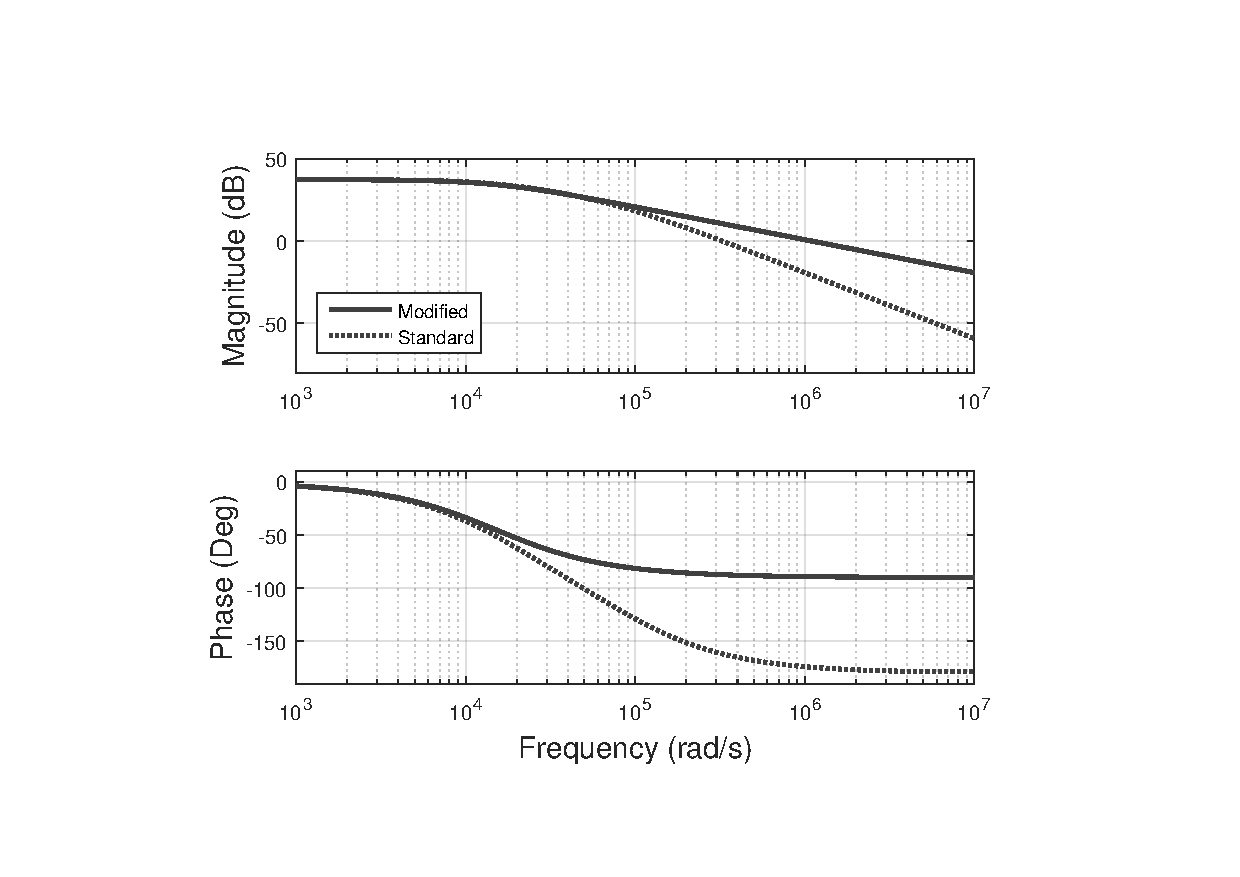
\includegraphics[width=0.8\textwidth]{cs_comparison}
		\caption{Bode plot of current source}
		\label{fig:uncomp-cs}
	\end{figure}
	Due to the removal of the output capacitor in the standard buck converter, the order of the system is reduced to one.
	
\section{Nonlinear Modelling}
	The approach described in the previous section relies on the approximation of switching phenomenon by duty ratio. Hence, a nonlinear model is derived for current and voltage sources based on the phase plane analysis.
	\subsection{Voltage Source Model}
    Figure \ref{fig:nl-1} depicts simplified two quadrant converter which constitutes the voltage source in the pulsed power topology. The resistances of inductor and capacitor shown are ignored for simplified mathematical treatment. To derive a nonlinear model of this converter, following choices of state variables are made.
    \begin{align*}
    	x_1 &= v - v_{ref} \\
    	x_2 &= \dot{x_1} = \frac{i_C}{C}
    \end{align*}
    Let the switch state if $Q_1$ be the input $u$ such that $Q_1$ is ON when $u = 1$ and OFF when $u = 0$. $Q_2$ is complementary to $Q_1$, hence, $Q_2$ is OFF when $u = 1$ and ON when $u = 0$. Applying Kirchhoff's Voltage Law for both the circuit states
    \begin{align*}
        u &= 1 \implies \dot{x_2} = -\frac{x_1}{LC} -\frac{V_{ref}}{LC} + \frac{V_{dc}}{LC}\\
        u &= 0 \implies \dot{x_2} = -\frac{x_1}{LC} -\frac{V_{ref}}{LC}
    \end{align*}
    Thus, the complete dynamics of the voltage source are
    \begin{align}
        \dot{x_1} &= x_2\\
        \dot{x_2} &= -\frac{x_1}{LC} + u\frac{V_{dc}}{LC} -\frac{V_{ref}}{LC}
        \label{eq:nl1}
    \end{align}
	\begin{figure}[h]
		\begin{subfigure}{.55\textwidth}
          \centering
          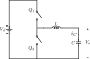
\includegraphics[width=0.9\linewidth]{nl-2quad-mod-master}
          \caption{Two quadrant converter}
          \label{fig:nl-1}
        \end{subfigure}
        \begin{subfigure}{.4\textwidth}
          \vspace{2cm}
          \centering
          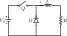
\includegraphics[width=0.9\linewidth]{nl-buck-mod-master}
          \caption{Single quadrant converter}
          \label{fig:nl-2}
        \end{subfigure}
		\caption{Nonlinear modelling circuit}
	\end{figure}

\subsection{Current Source Model}
    Figure \ref{fig:nl-2} shows simplified single quadrant converter which constitutes the current source in the pulsed power topology. To derive a nonlinear model of this converter, the state variable is chosen as
    \begin{align*}
    	x_1 = i - i_{ref}
    \end{align*}
    Let the switch state of $Q$ be the input $u$ such that $Q$ is ON when $u = 1$ and OFF when $u = 0$. Applying Kirchhoff's Voltage Law for both the circuit states
    \begin{align*}
        u &= 1 \implies \dot{x_1} = -\frac{R}{L}x_1 -\frac{R}{L}i_{ref} + \frac{V_{dc}}{L}\\
        u &= 0 \implies \dot{x_1} = -\frac{R}{L}x_1 -\frac{R}{L}i_{ref}
    \end{align*}
    Thus, the complete dynamics of the current source are
    \begin{align}
        \dot{x_1} &= -\frac{R}{L}x_1 + u\frac{V_{dc}}{L} -\frac{R}{L}i_{ref}
        \label{eq:nl2}
    \end{align}
\Chapter{Controller Design}
\label{chap:lincontrol}
	The dielectric strength of deionized water is around 70 MV/m. Therefore, if the gap is 1 $\mu$m, minimum voltage of 70 V is required to ensure the sparking. Keeping a sufficient margin, the control objectives for the power supply are as follows:
	\begin{enumerate}
		\item Voltage source must maintain a voltage $V_{\text{ref}}$ i.e. 80 V across its load terminals while rejecting load current disturbances up to $I_{\text{ref}}$ i.e. 10 A.
		\item Current source must provide a current of 10 A.
		\item Generating switching signal for $Q_d$ to control the erosion time during each machining cycle 
	\end{enumerate}
	The control objectives mentioned above are to be achieved by designing a scheme for switching the appropriate devices such that the aforementioned criteria is satisfactorily met. A PI controller is implemented and tuned using trial and error initially. However, this chapter describes a more systematic approach of compensator design based on the frequency response of the small signal transfer functions derived earlier. Automated K Factor approach \cite{muhamad2005design} used conventionally for power electronic converters has been found inadequate in this case. The removal of capacitor in current source and the load from the voltage source lead to different models than those for which this approach has been tested. Hence, the compensator design criteria are discussed here. A relatively advantageous technique of current mode control is also reviewed.

\section{Direct Duty Ratio Control}
	 A simple method to achieve this goal is varying the duty cycle of a pulse width modulated (PWM) signal with fixed frequency $F_s$. $F_s$ is the switching frequency of the MOSFETs used in the converters. A feedback loop is constructed by using a lead-lag compensator for this purpose as shown in figure \ref{fig:dirduty-1}.

	\begin{figure}[h]
		\centering
		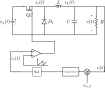
\includegraphics[width=0.6\textwidth]{direct-duty}
		\caption{Block diagram of direct duty ratio control of single quadrant converter}
		\label{fig:dirduty-1}
	\end{figure}

	For the two quadrant converter, since the control objective is tracking the reference voltage $v_{\text{ref}}$, the output voltage $v(t)$ is sensed. $v(t)$ is compared with $v_{\text{ref}}$ to obtain the error signal. This error signal is the representative of the deviation of current state of the system from the desired state. The design procedure followed is described next.

	To improve the transient response gain crossover frequency $\omega_{gc}$ should be maximum. But, to avoid resonance, it is chosen roughly an order on magnitude lower than the switching frequency. This is chosen as
	\begin{equation}
		\omega_{\text{cross}} = \dfrac{2 \pi F_s}{10}
		\label{eq:50}
	\end{equation}
    Also, the desirable range of phase margin is 45 to 60$^\circ$ \cite{book:768263}. Let the desired phase margin be $PM_{des}$.
    Phase that has to be added to the system is 
    \begin{equation}
    \phi_{m_1} = PM_{des} -\left(180 + \phi_{\text{OL}}\Bigr|_{\omega = \omega_{\text{cross}}}\right)
	\label{eq:50a}    
    \end{equation}
    The general form of compensator is 
    \begin{equation}
    	G_{\text{lead}} = \dfrac{1+a_1T_1s}{1+T_1s}
	    \label{eq:51}    
    \end{equation}
    where $a_1>1$
    The maximum phase lead due to this compensator is given by
    \begin{equation}
    	\phi_{m_1} = \sin^{-1}\left(\dfrac{a_1-1}{a_1+1}\right)
	    \label{eq:52}    
    \end{equation}
    This phase lag is added in between the corner frequencies $\dfrac{1}{T_1}$ and $\dfrac{1}{a_1T_1}$ and is maximum at
    \begin{equation}
    	\omega_{m_1} = \dfrac{1}{T_1\sqrt{a_1}}
	    \label{eq:53}    
    \end{equation}
    Thus, to make phase margin as desired at the gain crossover frequency as decided, $T_1$ and $a_1$ are chosen as
    \begin{equation}
		\begin{split}
			a_1 &= \dfrac{1+\sin(\phi_{m_1})}{1-\sin(\phi_{m_1})}\\
			T_1 &= \dfrac{1}{\omega_{m_1}\sqrt{a_1}}		
		\end{split}
		\label{eq:54}    
    \end{equation}
    To reduce the steady state error, a lag compensator $G_{\text{lag}}$ is required such that $\omega_{m_2} << \omega{\text{cross}}$. In the general form
    \begin{equation}
    	G_{\text{lag}} = \dfrac{1+a_2T_2s}{1+T_2s}
	    \label{eq:55}    
    \end{equation}
    where $0 < a_2 < 1$.
    The steady state gain added by this compensator is 
    \begin{equation}
    	\lim_{s\to\infty} \dfrac{1+a_2T_2s}{1+T_2s} = \dfrac{1}{a_2}
	    \label{eq:56}    
    \end{equation}
    Choosing a small enough $a_2$, $T_2$ has been found as
    \begin{equation}
		T_2 = \dfrac{1}{\omega_{m_2}\sqrt{a_2}}
		\label{eq:57}
    \end{equation}
    Finally, the loop gain is balanced by taking $K$ as
    \begin{equation}
		K = \Bigl| \dfrac{1}{G_{\text{lag}} G_{\text{lead}} G_{\text{OL}}} \Bigr|_{\omega = \omega_{\text{cross}}}
		\label{eq:58}
    \end{equation}
    The final controller is
    \begin{equation}
		G_c(s) = K G_{\text{lag}} G_{\text{lead}}
		\label{eq:59}
    \end{equation}
    The bode plot for compensated open loop transfer function of the voltage source is shown in figure \ref{fig:comp-vs}
	\begin{figure}[h]
		\centering
		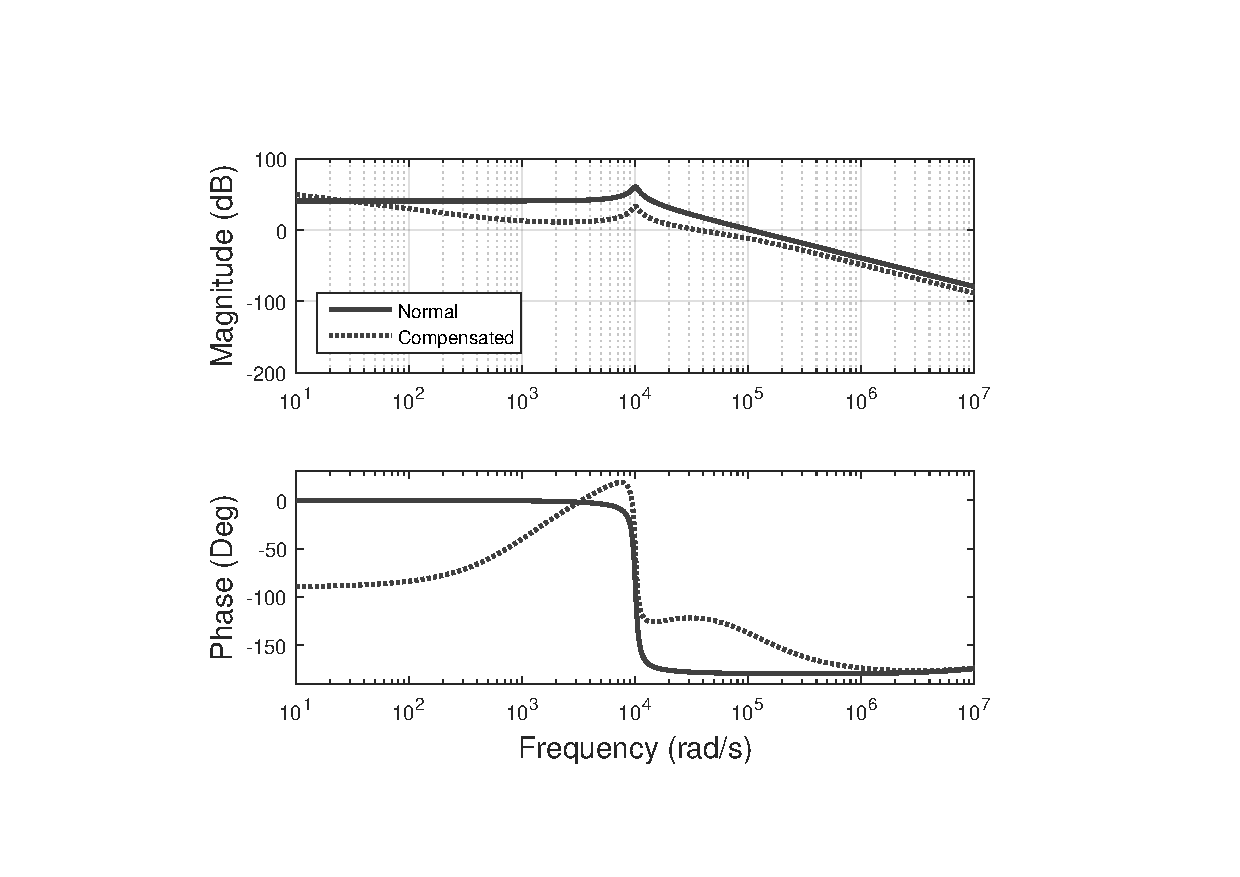
\includegraphics[width=0.8\textwidth]{vs_compesator_bode}
		\caption{Bode plot of compensated transfer function of voltage source}
		\label{fig:comp-vs}
	\end{figure}
	For the current source, phase margin is already sufficient, so closing the negative feedback loop with unity should be enough. This has been verified in the simulation. Figure \ref{fig:comp-cs} shows the bode plot obtained by following the same process as the previous.
	\begin{figure}[H]
		\centering
		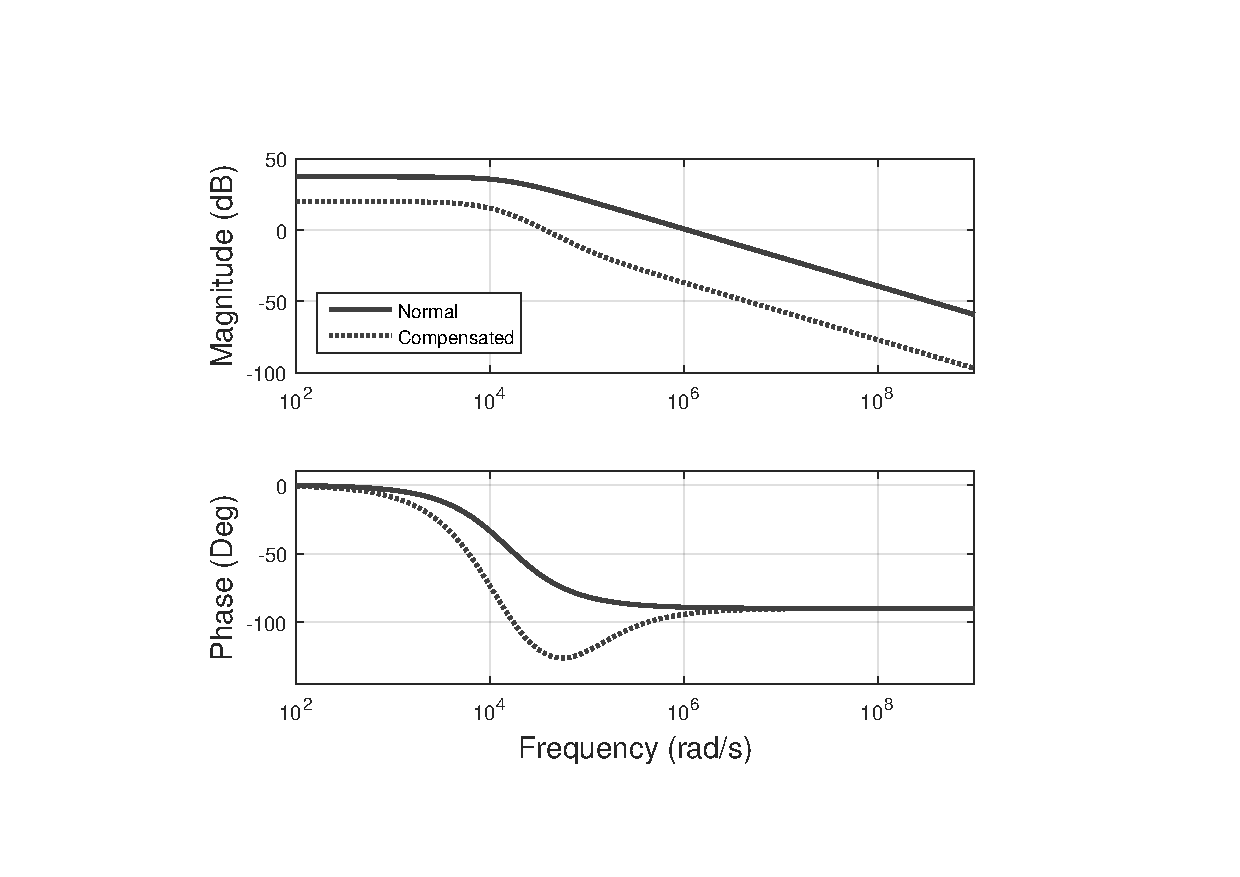
\includegraphics[width=0.8\textwidth]{cs_compesator_bode}
		\caption{Bode plot of compensated transfer function of current source}
		\label{fig:comp-cs}
	\end{figure}

\section{Current Mode Control}
	Converters employing direct duty ratio control require a separate protection against over current for each switch. However, if the control method is based on the peak current through switch, then the requirement for such a protection effort is eliminated as the current is not allowed to rise above a particular threshold in each switching cycle. Also, the dynamics of such a controller are much simple than the direct duty ratio control. This section describes peak current mode control \cite{book:941109}, loosely referred to as current mode control, which employs this method to achieve the output current or voltage tracking objective.

	\begin{figure}[h]
		\centering
		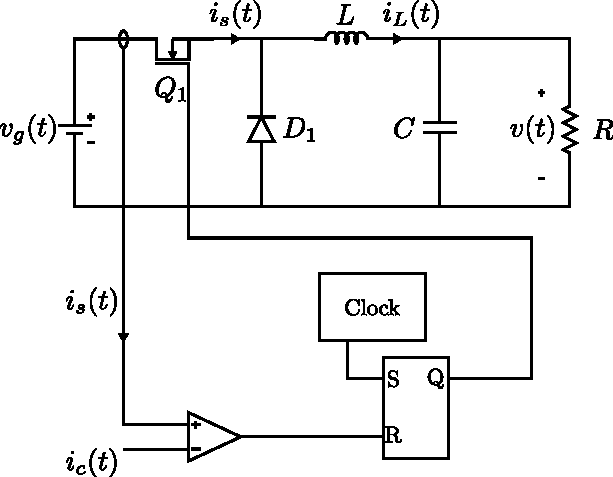
\includegraphics[width=0.6\textwidth]{current-mode-minimal-master}
		\caption{Block diagram of current mode control of single quadrant converter}
		\label{fig:16}
	\end{figure}

	Figure \ref{fig:16} represents the block diagram for current mode control of a single quadrant converter. At the start of each switching cycle of frequency $F_s$, $Q_1$ is switched on by a clock pulse which sets the latch in a high state. The switch remains in the on state until a reset pulse is applied to the latch. During on time, the current $i_s(t)$ through $Q_1$ rises with slope $m_1$ as shown in figure \ref{fig:17}. When $i_s(t)$ reaches the control current $i_c(t)$, the comparator, being non inverting in nature, generates a reset pulse for the latch which turns the switch off. For the remainder of the switching period, the current through switch is zero. If the inductor $L$ is chosen such that the continuous conduction mode operation is ensured around $i_c(t)$, then the current through the inductor decreases at a rate of $-m_2$ during the off time to a value of $i_L(T_S)$ at $T_s$ as shown in figure \ref{fig:18}.

	\begin{figure}[h]
	\begin{subfigure}{0.49\textwidth}
		\centering
		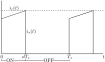
\includegraphics[width=\linewidth]{switch-current}
		\caption{Switch current}
		\label{fig:17}
	\end{subfigure}
	\begin{subfigure}{0.49\textwidth}
		\centering
		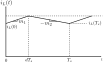
\includegraphics[width=\linewidth]{inductor-current}
		\caption{Inductor current}
		\label{fig:18}
	\end{subfigure}
	\caption{Switch and inductor currents in current mode control}
	\end{figure}

	The slopes $m_1$ and $-m_2$ are given by \cite{book:941109}
	\begin{align}
		m_1 = \dfrac{v_g-v}{L} \quad \text{and} \quad  -m_2=\dfrac{v}{L}
		\label{eq:1}
	\end{align}
	where $v_g$ is the dc link voltage, $v$ is the output voltage, and $L$ is the value of inductor of the buck converter.
	During on time, inductor current at $t=dT_s$, $\hat{i}_L(dT_s)$ in terms of slope $m_1$ is given by
	\begin{equation}
		i_L(dT_s) = i_c = i_L(0)+m_1dT_S
		\label{eq:2}
	\end{equation}
	During the off time, the inductor current at $t=T_s$ is 
	\begin{equation*}
		i_L(T_s) = i_L(dT_s) - m_2(1-d)T_S
	\end{equation*}
	Substituting $i_L(dT_s)$ from equation \eqref{eq:1} in this relation results in
	\begin{equation}
		i_L(T_s) = i_L(0)+m_1dT_S - m_2(1-d)T_S
		\label{eq:3}
	\end{equation}
	At steady state, $m_2=M_2$, $d=D$, $i_L(0) = i_L(T_s)$, $m_1=M_1$, and . From equations \eqref{eq:2} and \eqref{eq:3}, at steady state
	\begin{equation*}
		0 = M_1DT_S - M_2(1-D)T_S
	\end{equation*}
	\begin{equation}
		\dfrac{M_2}{M_1} = \dfrac{D}{1-D}
		\label{eq:4}
	\end{equation}

	This method requires additional current sensing circuit as compared to duty ratio control methods, but in practice, duty ratio control methods also require current sensing circuit for protection against over currents. This method exploits the available current sensors which would otherwise be operating independently from the control scheme to achieve the control objective. Switch failures due to excessive currents are avoided by saturating the peak control signal $i_c(t)$ thus ensuring that the switch will turn off when excessive current flows through it during each switching period.

	A drawback of this method is its high noise sensitivity. Perturbations in sensed switch current can cause premature turn off of the switch. Also, converter becomes unstable even for small perturbations in switch current when operating on duty cycles greater than 50\% as the perturbation increases in magnitude in each subsequent switching cycle. However, this can be remedied by adding a ramp to the observed switch current. The intuition behind this is explained in appendix \ref{app:instability-cmc}.
	\begin{figure}[h]
		\centering
		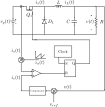
\includegraphics[width=0.6\textwidth]{current-mode-voltage-control}
		\caption{Controlled voltage source using current mode control}
		\label{fig:24}
	\end{figure}
	For the two quadrant converter, an outer voltage feedback loop is constructed on top the current mode controller as shown in figure \ref{fig:24}. A small signal model of the converter is derived under a justifiable assumption for this purpose. If the magnitude of the ramp and that of the inductor current ripple are less, the mean inductor current $i_L$ tracks the reference $i_c$. Thus, the current mode controller designed above operates ideally under these conditions. Therefore, the inductor current transfer function is $\dfrac{i_L}{i_c} \approx 1$. The current mode control part of this controller can be replaced by an ideal current source of magnitude $i_c(t)$ and an equivalent circuit can be constructed as shown in figure \ref{fig:25}
	%It is assumed that the current mode controller operates ideally, and hence causes the average inductor current ${i}_L$ to be identical to the control ${i}_c$. This approximation is justified whenever the inductor current ripple and artificial ramp have negligible magnitudes. The inductor current then is no longer an independent state of the system because $\dfrac{i_L}{i_c} \approx 1$.
	\begin{figure}[h]
		\centering
		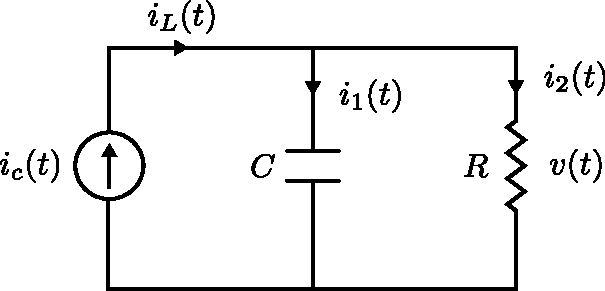
\includegraphics[width=0.5\textwidth]{modelling}
		\caption{Current mode control replaced as current source in buck converter}
		\label{fig:25}
	\end{figure}
	From Kirchhoff's Current Law, the output current of the current source is
	\begin{equation}
		i_c(t) = C\dfrac{dv(t)}{dt} + \dfrac{v(t)}{R}
		\label{eq:cmc-1}
	\end{equation}
	Let the steady state value of the output current and output voltage be $I_c$ and $V$ respectively. If a small perturbation of magnitude $\hat{i}_c(t)$ is introduced in the current $i_c(t)$, the output voltage $v(t)$ gets perturbed by a magnitude of, say, $\hat{v}(t)$, then
	\begin{align}
		i_c(t) &= I_c + \hat{i_c}(t)\\
		v(t) &= V + \hat{v}(t)
		\label{eq:cmc-2}
	\end{align}
	From \eqref{eq:cmc-1},
	\begin{equation}
		I_c + \hat{i_c}(t) = C\dfrac{d}{dt}(V + \hat{v}(t)) + \dfrac{V + \hat{v}(t)}{R}
		\label{eq:cmc-3}
	\end{equation}
	At the steady state, 
	\begin{equation}
		\dfrac{dV}{dt} = 0 \quad \text{and} \quad I_c = \dfrac{V}{R}
		\label{eq:cmc-4}
	\end{equation}
	Therefore,
	\begin{equation}
		\hat{i_c}(t) = C\dfrac{d\hat{v}(t)}{dt} + \dfrac{\hat{v}(t)}{R}
		\label{eq:cmc-5}
	\end{equation}
	Taking Laplace transform
	\begin{equation}
		\hat{i}_c(s) = sC\hat{v}(s) + \dfrac{\hat{v}(s)}{R}
	\end{equation}
	\begin{equation}
		\dfrac{\hat{v}(s)}{\hat{i}_c(s)} = \dfrac{R}{1+sRC}
	\end{equation}
	This transfer function represents the first order dynamics. Thus, the simpler dynamics in comparison to models required for direct duty ratio control. A PI controller is used to complete the feedback loop to derive a controlled voltage source from a current mode controlled converter.
	
	\section{Pulsed Reference Scheme}
	The majority of the losses in the proposed converter are due to switches. Moreover, since the machining duty is about 10\% of the complete machining cycle, the ignition switch remains closed for 90\% of the time. When the ignition switch is turned ON, the current source delivers 10 A current through it. Thus, the losses during this period are $V_{Q_{d ON}}\times I_{ref}$. However, the value of current through ignition switch can be reduced during this period to reduce the losses. A pulsed reference scheme is proposed for the same as given below.
	\begin{figure}[h]
		\centering
		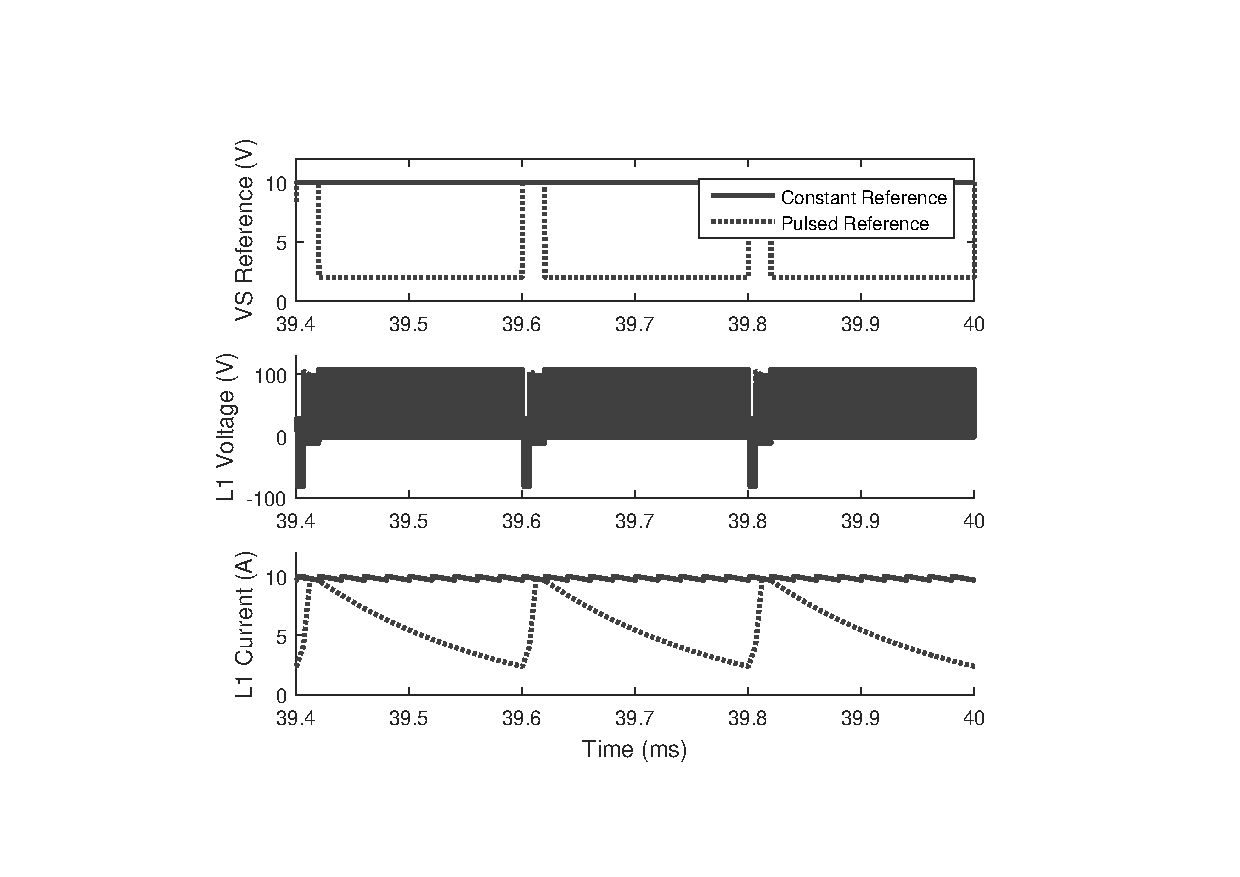
\includegraphics[]{power_comparison}
		\caption{Power comparison in pulsed reference scheme}
		\label{fig:pulsed-reference}
	\end{figure}
	The reference of the current source is pulsating between 10 A and 2 A instead of continuous 10A. When the machining duty period is completed the reference is lowered and maintained at this value until the machining cycle is complete. The reference is raised again just before the next machining cycle is initiated. This sequence of alternating references ensures that the current through ignition switch is considerably lower, thus reducing the $V_{Q_{d ON}}\times I_{ref}$ losses. Figure \ref{fig:pulsed-reference} shows the comparison of the voltage and current across the inductor under the pulsed and continuous reference schemes. The current through the ignition switch is governed by the inductor value. A low enough inductor value will ensure that the current through ignition switch decreases as the reference is lowered. It is verified in the simulations that inductor value of 100 $\mu$H is adequate for the pulsed reference scheme to cause a reduction of about 30\% in the overall converter power consumption.
	
	
	\section{Nonlinear Control}
	The linear controllers as discussed in the previous chapters are based on approximation of the system dynamics in the neighbourhood of an equilibrium point. These controllers work satisfactorily if the system is operated close to this equilibrium point, however,  the response is not guaranteed for operating points away from the equilibrium. If the reference for the system under consideration is not fixed, separate controllers may be required for each case. 
    
    The small signal model derived in chapter \ref{chap:modelling} relates the output voltage and current to the duty of switches. The time averaging and small signal perturbation techniques used to derive this model are based on the assumptions that converter will operate close to the reference value at all times. This can result in restriction on the voltage and current ranges of the pulsed power supply. Hence, a nonlinear control technique is proposed in the following sections.
    
    Nonlinear controllers preserve the dynamic performance over wide range of operation. This section elaborates on Sliding Mode Control of the individual converters in the pulsed power supply topology.

\subsection{Sliding Mode Control}
    Figure \ref{fig:nl-3} shows the phase portrait of the voltage source. In this representation, each point is a state vector $(x_1,x_2)$ where $x_1$ is represented along X-axis and $x_2$ is represented along Y-axis. The arrows at each point represent the vector of derivatives of the states $(\dot{x_1},\dot{x_2})$. In this figure, the magnitude of $\dot{x_1}$ is scaled by a factor of $1/LC$ to limit the overlapping of arrows due to $|\dot{x_1}| >> |\dot{x_2}|$ for the practical values of $L = 2$ mH and $C = 100$ $\mu$F. The two focii of this phase portrait are presented by asterisks. If the system starts from an initial state $(x_{10},x_{20})$ with $u_0$ as its input, it will move along the arrows as these represent the direction of the change in the states for the particular input.
    \begin{figure}[h]
      \centering
      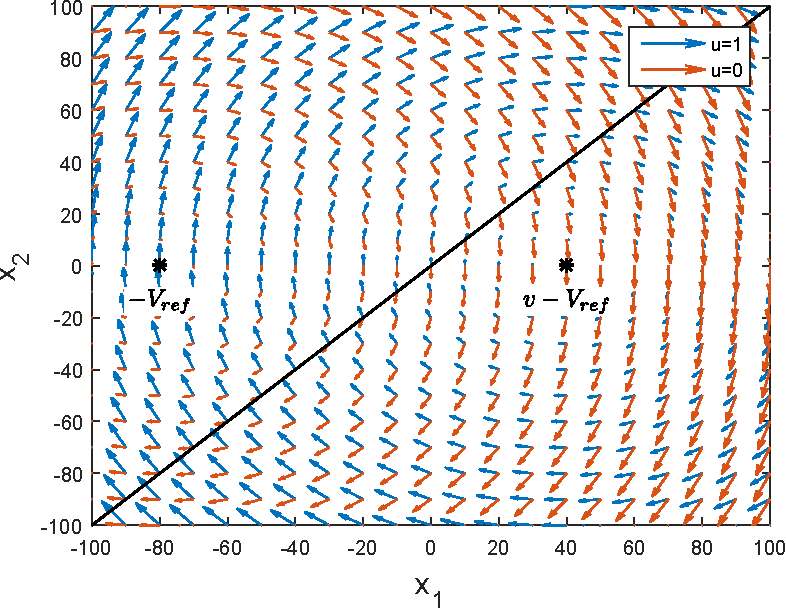
\includegraphics[width=0.7\linewidth]{phase_map}
      \vspace{-0.5cm}
      \caption{Phase portrait of voltage source}
      \label{fig:nl-3}
	\end{figure}
	Consider a surface $\sigma (x) = c x_1 + x_2 = 0$ represented by a straight line in figure \ref{fig:nl-3}. If the dynamics are restricted to this this surface only, the states converge to the equilibrium point $(0,0)$ when $c > 0$. This is due to the fact that $x_2 = \dot{x_1}$ and the dynamics on the surface are $\dot{x1} = -c x_1$. As a result, the system moves towards equilibrium point when it is on this surface. This surface is called the sliding mode. In general, for a $n$ dimensional system the sliding surface is a $n-1$ dimensional hyperplane.
	
	Design of a sliding mode control involves determining a suitable input which will make the sliding mode reachable from any point in the state space. In other words, if system is started from any state and the control law is followed, the system should reach this sliding surface. Further, any deviations from this surface should result in such an input which will push the system towards the same sliding surface.
	
	From figure \ref{fig:nl-3}, it is evident that following the input $u=0$ whenever the state is above the sliding surface \cite{spiazzi1997sliding} i.e. $\sigma (x) > 0$ and $u=1$ when the state is below the sliding surface i.e. $\sigma (x) < 0$ makes the sliding surface reachable. This choice of inputs is not unique, the can be other functions which can achieve the same purpose. Thus, the sliding mode control law can be summarised as
    \begin{align}
    	\begin{split}
	        u &= 1 \quad if \quad \sigma (x) < 0\\
	        u &= 0 \quad if \quad \sigma (x) > 0
	        \label{eq:nl-3}
	    \end{split}
    \end{align}
    \begin{figure}[h]
      \centering
      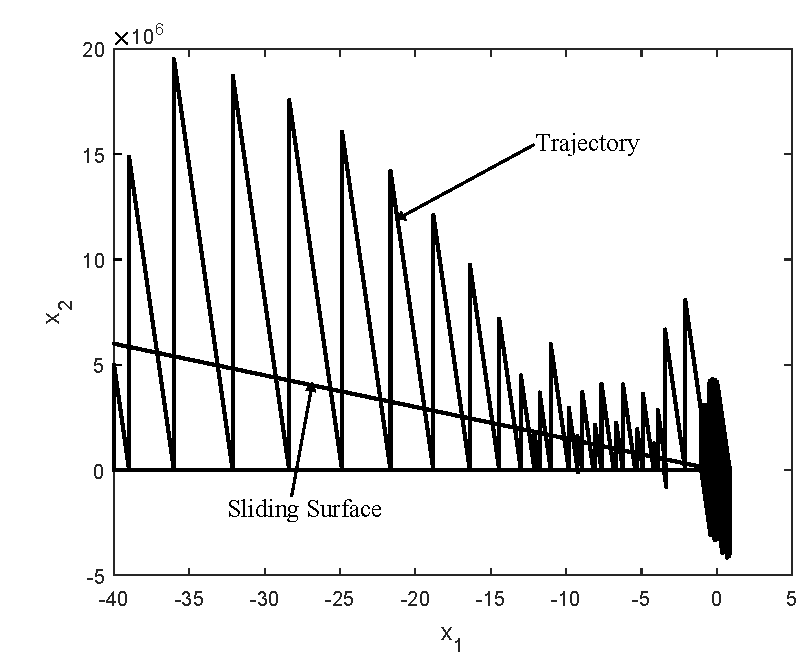
\includegraphics[width=0.6\linewidth]{vs-trajectory}
      \vspace{-0.5cm}
      \caption{Trajectory of voltage source}
      \label{fig:nl-4}
	\end{figure}
    Figure \ref{fig:nl-4} shows the trajectory followed by the simulated two quadrant converter to achieve the reference of 40 V. The sliding surface used for this controller is represented by a straight line. Initially the system oscillates around this sliding surface while moving closer to the equilibrium point with each oscillation. The magnitude of oscillations also decreases gradually to a small fixed value. The oscillations don't die out completely because of the finite sampling and actuation time constraints of the practical systems.

\subsection{Controller Implementation}
    \begin{figure}[h]
      \centering
      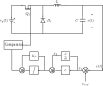
\includegraphics[width=0.6\linewidth]{sliding-mode}
      \caption{Implementation of sliding mode controller}
      \label{fig:nl-5}
	\end{figure}
	Figure \ref{fig:nl-5} shows one implementation of the sliding mode controller. A subtractor is used to calculate the state $x_1$ which is then differentiated to obtain the state $x_2$. A summer is used to obtain the value of the sliding parameter $\sigma(x)$. However, most practical systems employ a PI controller over $\sigma(x)$.
	
	From the phase plane in figure \ref{fig:nl-3}, the gradient vectors for both the inputs are co-linear along the X-axis. However, the point where their magnitudes balance each other is not at the equilibrium point. The vector sum of both the gradients is zero at a point slightly to the left of equilibrium point. This can be confirmed from the trajectory in figure \ref{fig:nl-4} and the controller is found to be stabilised when $x_1=-5$ if integrator is not used. At this point, the trajectory ceases any movement along the X-axis, hence, the steady state error. The system continues oscillation along Y direction only as both the gradients are parallel to Y-axis and have equal magnitude.
	
	Introduction of PI action \cite{spiazzi1997sliding} on the sliding parameter causes its value to accumulate over time thus biasing the $cx_1$ term while $\dot{x_1}$ remains the same resulting in delayed corrective action. Finally, a comparator is used to compare the sliding parameter value and provide a suitable input to the switch. Constant switching frequency is not an issue with discrete controllers as this algorithm can be executed at a precise rate via timed interrupts and so ignored in this particular realisation. 
    \begin{figure}[h]
        \begin{subfigure}{.49\textwidth}
            \centering
            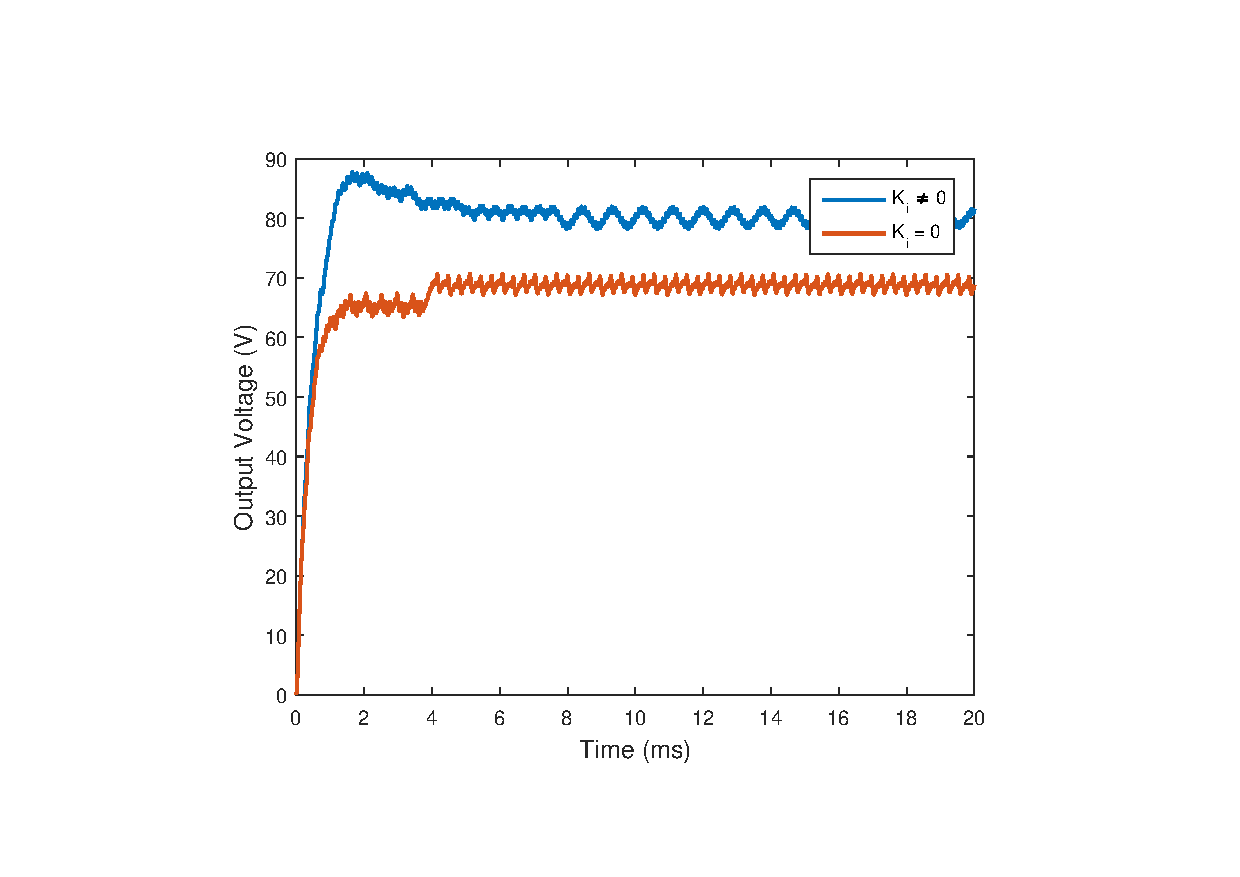
\includegraphics[width=\linewidth]{nl-response}
            \caption{Voltage source response}
            \label{fig:nl-6}
        \end{subfigure}
        \begin{subfigure}{.49\textwidth}
            \centering
            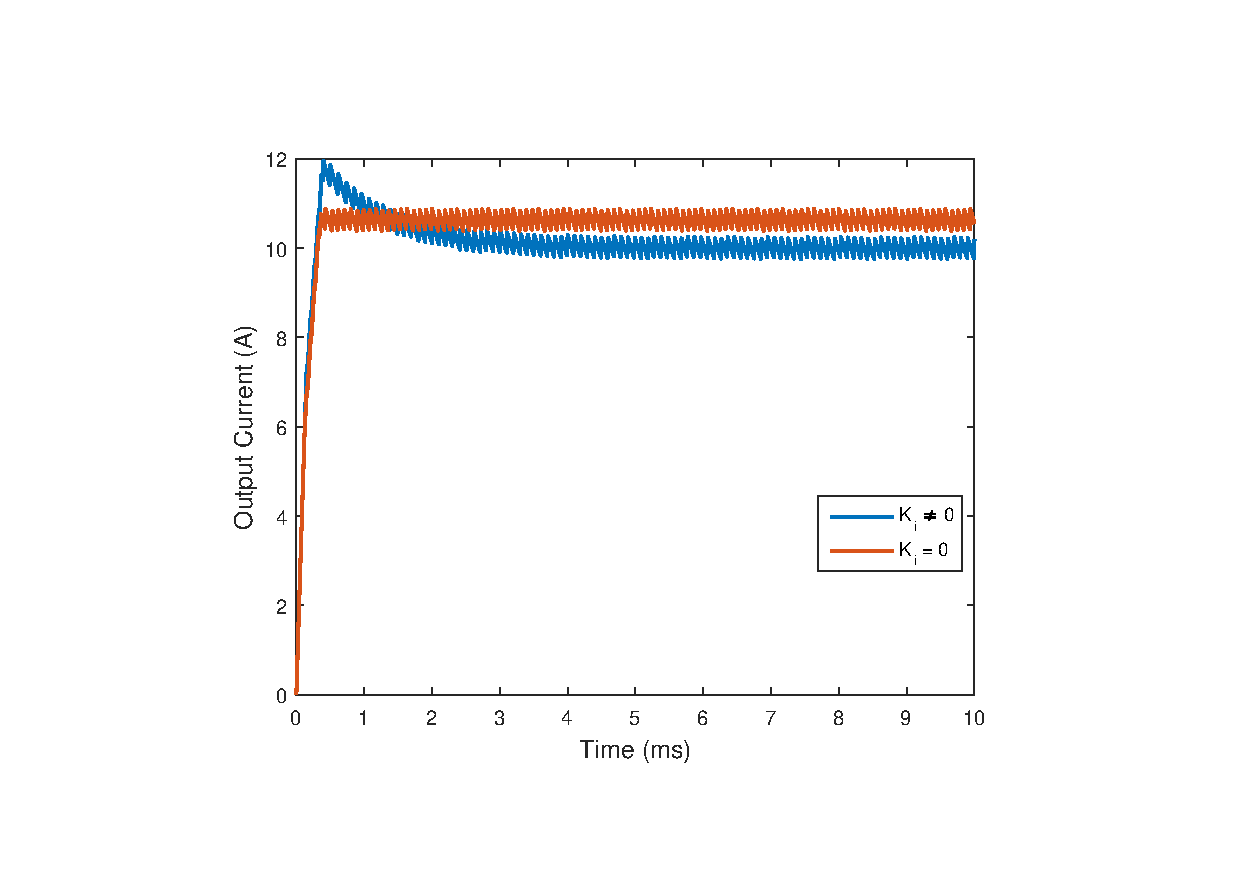
\includegraphics[width=\linewidth]{nl-cs-response}
            \caption{Current source response}
            \label{fig:nl-7}
	    \end{subfigure}
	    \caption{Step response of sliding mode controllers}
	\end{figure}
	Figure \ref{fig:nl-6} and figure \ref{fig:nl-7} show the simulated step response of voltage and current sources respectively operating via sliding mode controllers. The voltage source reference is 80 V and the current source reference is 10 A. The operation without the PI action on sliding surface is also shown to compare the performance with the proposed modification to the implementation.

\Chapter{Hardware Implementation}
\label{chap:hardware}
    The pulsed power supply is implemented using three IGBT modules. The other major hardware components required in this setup are inductors, capacitors and DC power source. The current and voltage sensing have been achieved with the shunt resistors and conditioning circuit. The control algorithm has been implemented on a Texas Instruments F28069 Launchpad. This chapter deals with the methodology used to arrive at the capacitor and inductor sizes suitable for pulsed power application. The complete hardware implementation of the converter topology is presented along with the necessary interfacing and sensing circuits.
	figure \ref{fig:block-diag} shows the top level organisation of the complete hardware setup.
    \begin{figure}[h]
        \centering
        \includegraphics[width=0.8\textwidth]{ConvSch}
        \caption{Block Diagram of Hardware Setup}
        \label{fig:block-diag}
    \end{figure}

\section{Sizing of Passive Components}
\subsection{Inductor Selection}
	The purpose of inductor in DC-DC switched power supplies is to maintain the current when the DC link switch is off i.e. to reduce the ripple in output voltage or current depending on the converter. With this criteria, the inductor value should be high, but when a large inductor is used, the rise time of converter is more as it takes more time for the current to rise. Hence, the selection of inductor is trade-off between the current ripple and transient response of the converter. 

	For the single quadrant converter which is used as current source, criteria for selection of inductor value is taken to be the the inductor current ripple. The relation between inductor value and this ripple \cite{book:768263} is 
	\begin{equation}
		\Delta I_L = \dfrac{V_{o1}}{L_1} (1-D) T_s
		\label{eq:ind-1}
	\end{equation}
	where $V_{o1} = I_{\text{ref}} R_L$ is the output voltage of the single quadrant converter, $L_1$ is the value of the inductor, $D$ is the steady state duty cycle of the converter, $\Delta I_L$ is the ripple in in inductor current and $T_s = \dfrac{1}{F_s}$ is the switching period.
	\begin{equation}
		L_1 \geq \dfrac{V_{o1}(V_d-V_{o1})}{\Delta I_L F_s V_d}
		\label{eq:ind-1a}
	\end{equation}
	Based on these calculations, inductor $L_1$ must be grater than 2 mH. 

	For the voltage source, the boundary condition for continuous conduction mode operation governs the choice of inductor. Because the output current need not be controlled here, the ripple criteria is relaxed in favour of ensuring the continuous conduction mode of the current source. This is ensured whenever the following criteria is satisfied \cite{book:768263}
	\begin{equation}
		I_{L_2} \geq \dfrac{DT_s}{2L_2}(V_d-V_{o2})
		\label{eq:ind-2}
	\end{equation}
	If the average inductor current $I_{L_{\text{avg}}}$ becomes less than this boundary value, the converter operates in discontinuous mode. To extend the range of operation of the converter to lower average currents, the inductor is chosen such that continuous conduction mode is ensured at the lowest extreme of the intended range of operation. For satisfactory operation \cite{muhamad2005design} at $\dfrac{1}{5}I_{L_2}$, the condition in inequality \eqref{eq:ind-1} is
	\begin{equation}
		\dfrac{1}{5}I_{L_2} \geq \dfrac{DT_s}{2L_2}(V_d-V_{o2})
		\label{eq:ind-3}
	\end{equation}
	where $I_{L_2} = V_d / R_L$, $D$ is the steady state duty cycle, $T_s = 1 / F_s$ is the switching period, $L_2$ is the inductor value, and $V_d$ and $V_o = V_{\text{ref}}$ are the DC link and converter output voltages respectively. 
	Therefore,
	\begin{equation}
		L_2 \geq 2.5\dfrac{DT_s}{I_{L_2}}(V_d-V_{\text{ref}})
		\label{eq:ind-4}
	\end{equation}
	Based on this relation the inductor for voltage source must be greater than 0.15 mH.

\subsection{Capacitor Selection}
	Capacitor is required in the output stage of two quadrant converter to filter out the output voltage ripple. For a ripple of $\Delta V_{o2}$, the value of capacitor required is given by\cite{book:768263}
	\begin{equation}
		C_2 \geq \dfrac{\Delta I_{L_2}T_s}{8\Delta V_{o2}}
		\label{eq:ind-4a}
	\end{equation}
	The current ripple is given by,
	\begin{equation}
		\Delta I_{L_2} \geq \dfrac{V_{o2}}{L_2}(1-D) T_s
		\label{eq:ind-4b}
	\end{equation}
	Here, $V_{o2} = V_{\text{ref}}$ and $T_s = 1 / F_s$,
	\begin{equation}
		C_2 \geq \dfrac{1 - D}{8 \dfrac{\Delta V_{o2}}{V_{\text{ref}}}L_2 F_s^2}
		\label{eq:ind-5}
	\end{equation}
	The capacitor must be larger than $10 \mu F$.
	
\subsection{Trajectory based selection of L and C}
    The above calculations only provide a desired range of the inductors and capacitors. This treatement is enough for design of standard DC-DC converters. But, in the proposed pulsed power supply, the current source output will act as disturbance to the voltage source once the ignition switch is opened. To withstand these disturbances the value of inductor and capacitor must account for the settling time and stability.
	\begin{figure}[h]
	\begin{subfigure}{\textwidth}
		\begin{subfigure}{0.49\textwidth}
		\centering
			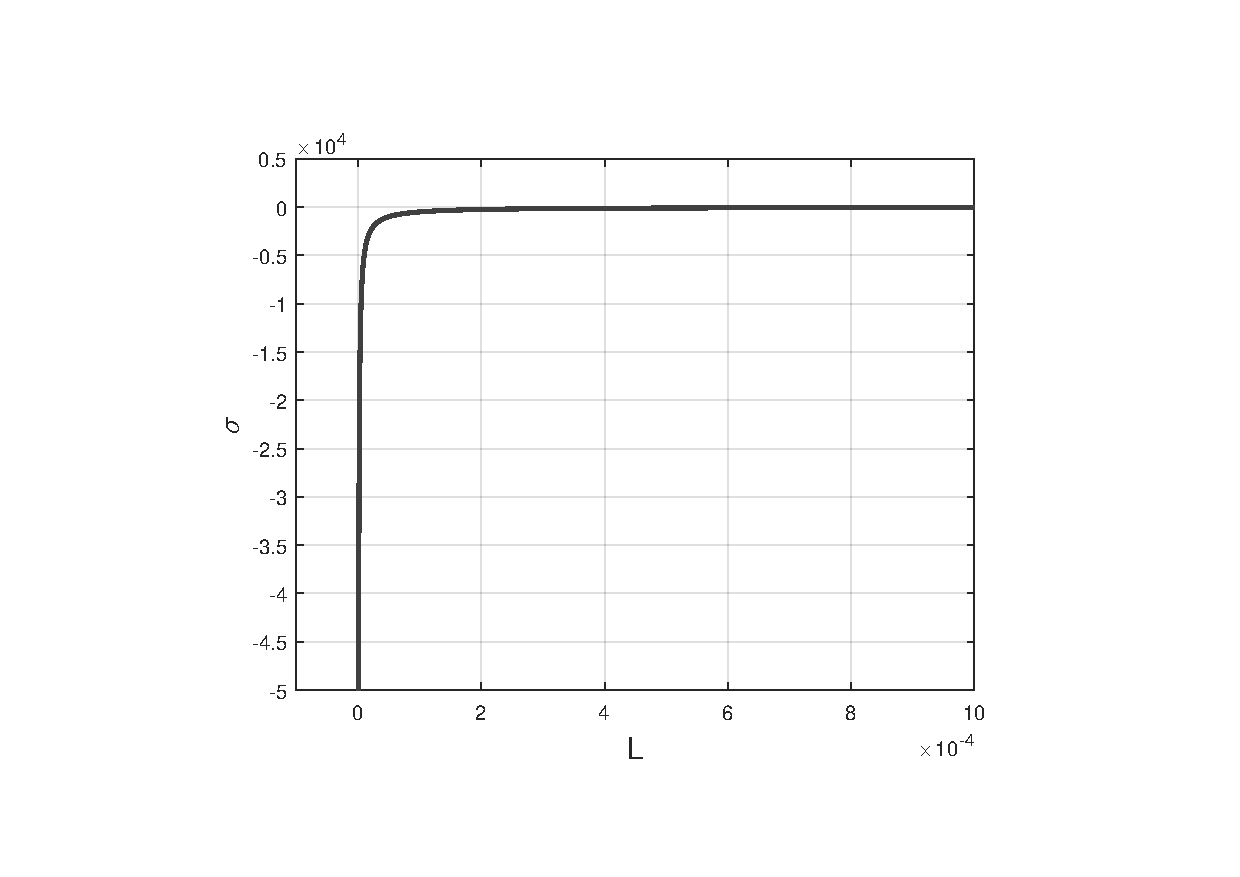
\includegraphics[width=\linewidth]{pd_real_vs_l2}
			\caption{$\sigma$ vs $L_2$}
			\label{fig:pd_real_vs_l2}
		\end{subfigure}
		\begin{subfigure}{0.49\textwidth}
			\centering
			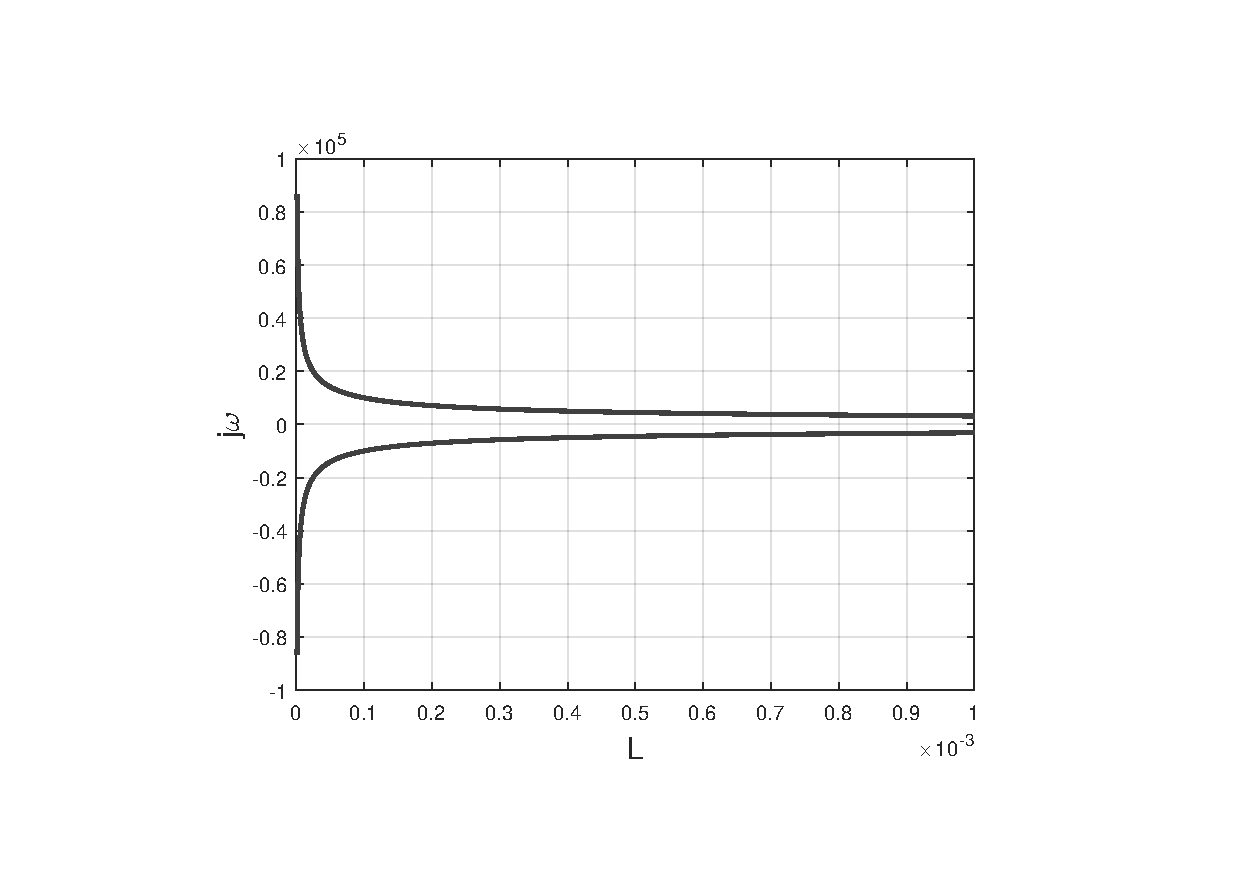
\includegraphics[width=\linewidth]{pd_imag_vs_l2}
			\caption{$j\omega$ vs $L_2$}
			\label{fig:pd_imag_vs_l2}
		\end{subfigure}
	\end{subfigure}
	\begin{subfigure}{\textwidth}
			\begin{subfigure}{0.49\textwidth}
			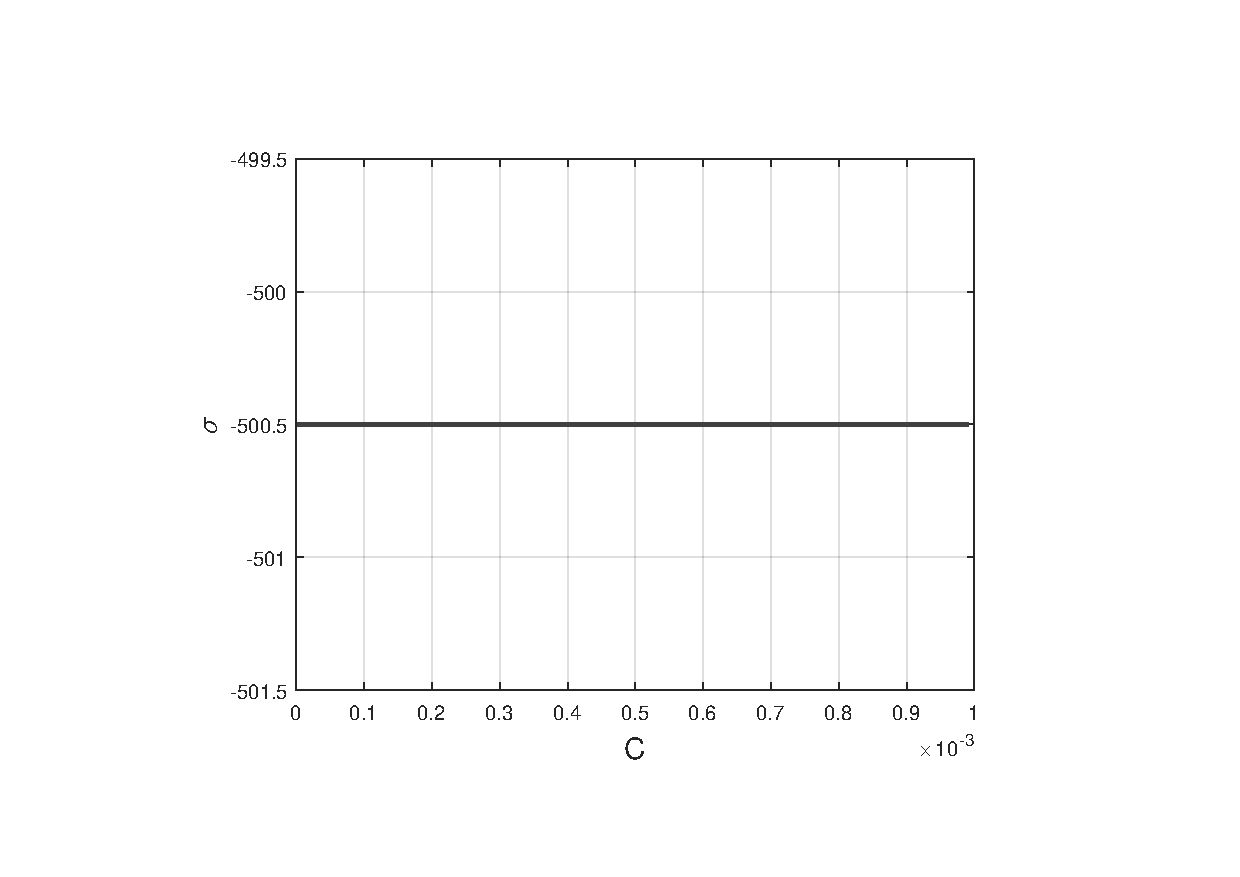
\includegraphics[width=\linewidth]{pd_real_vs_c2}
			\caption{$\sigma$ vs $C_2$}
			\label{fig:pd_real_vs_c2}
		\end{subfigure}
		\begin{subfigure}{0.49\textwidth}
			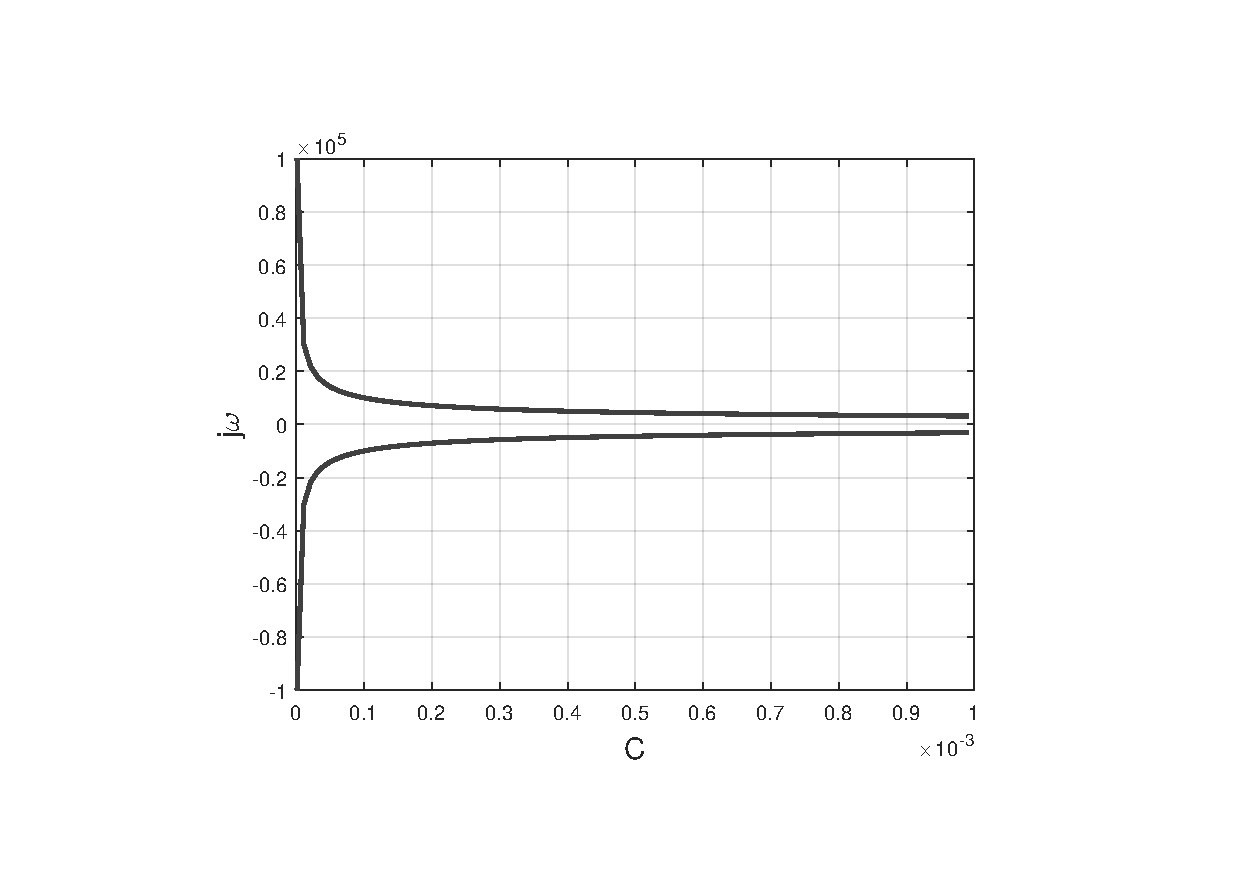
\includegraphics[width=\linewidth]{pd_imag_vs_c2}
			\caption{$j\omega$ vs $C_2$}
			\label{fig:pd_imag_vs_c2}
		\end{subfigure}
		\caption{Voltage source pole locus}
	\end{subfigure}
	\end{figure}
	Figure \ref{fig:pd_real_vs_l2}, figure \ref{fig:pd_real_vs_l2}, figure \ref{fig:pd_real_vs_c2}, and figure \ref{fig:pd_imag_vs_c2} depict the behavior of poles of the voltage source as the values of inductor and capacitor are changed. These plots are evident that the capacitor has no effect on the real part of the poles whereas the inductor influences bot the real and imaginary parts of the voltage source poles. As the capacitance increases, the imaginary part of the poles decreases nearly exponentially. This means that, increasing the capacitor value will reduce the oscillations, and hence improve the response to the disturbances.
	
	As the value of inductor is increased, the real part of the poles increases while the imaginary part of the poles decreases.  However, it is worth noting that the value of real part of the poles is always negative, so the converter is inherently stable. This implies that the value of inductor is a trade-off between the real and imaginary part of the poles. In other words, if the value of inductor is increased the response should become slower but the magnitude of oscillations due to disturbance would also decrease.
	\begin{figure}[h]
		\centering
		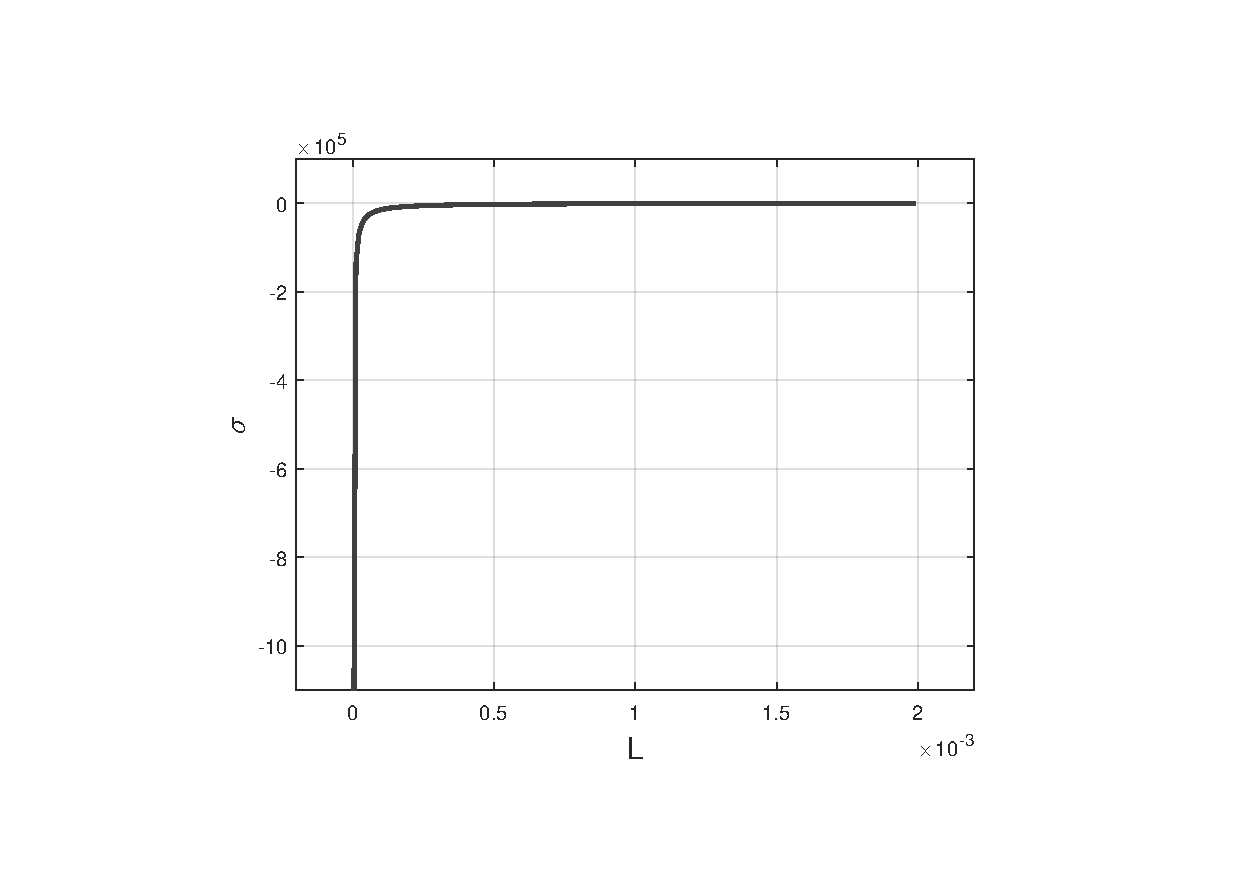
\includegraphics[width=0.6\linewidth]{pd_cs_l1}
		\caption{Current source pole locus: $\sigma$ vs $L_1$}
		\label{fig:pd_cs_l1}
	\end{figure}
	Figure \ref{fig:pd_cs_l1} shows the variation of the only pole of the current source with the value of inductor. As the value of inductor is decreased the response time of the current source decreases while the ripple increases. This fact is particularly useful in pulsed reference scheme discussed in chapter \ref{chap:lincontrol}. The current source must have a low enough rise time to respond to the pulsating reference. This has been verified via simulations.
	
	Based on the above discussion an inductor of 100 $\mu$H has been selected for current source and that of 2 mH for the voltage source during the practical implementation. A 1000 $\mu$F has been selected for the voltage source.	

\subsection{Snubber Design}
	Snubber is required across the ignition switch $Q_d$ to limit the over-voltage arising due to opening of the switch. In highly inductive circuits, when switch is opened, the path for current flow is broken. Therefore, a high voltage spike appears on the switch terminals due to large magnitude of $L\dfrac{di}{dt}$. Energy absorbing circuit like the snubber circuit, reduces these spikes. This section explains the design procedure for a R-C snubber used in parallel with the ignition switch $Q_d$.

	The peak current through the snubber circuit is given by
	\begin{equation}
		I_p = \dfrac{V_{oc}}{R_s}
		\label{eq:snub-1}
	\end{equation}
	where $V_{OC}$ is the open circuit voltage across the switch, $R_s$ is the snubber resistance and $I_p$ is the peak current through the snubber.

	The current flowing through $Q_d$ before interruption is $I_{\text{ref}}$ and the maximum voltage across the terminals of $Q_d$ is $V_{\text{ref}}$. Hence, the snubber resistance $R_s$ should be minimum of
	\begin{equation}
		R_s \geq \dfrac{V_{\text{ref}}}{I_{\text{ref}}}
		\label{eq:snub-2}
	\end{equation}
	The snubber capacitance should be such that:
	\begin{enumerate}
		\item Energy that is allowed to be stored in the capacitor should be greater than the energy stored in the inductor i.e.
			\begin{align}
				\dfrac{1}{2}C_sV_{oc}^2 &\geq \dfrac{1}{2}L_{eq}I_p^2\\
				\therefore C_s &\geq \dfrac{L_{eq}I_p^2}{V_{oc}^2}
				\label{eq:snub-3}
			\end{align}
		\item The snubber time constant must not exceed the minimum ON time of $Q_d$. So, for time constant of snubber circuit to be 10\% of the on time of $Q_d$
			\begin{align}
				R_sC_s &\leq \dfrac{T_{on}}{10}\\
				\therefore C_s &\leq \dfrac{T_{on}}{10R_s}
				\label{eq:snub-4}
			\end{align}
	\end{enumerate}
	From equations \eqref{eq:snub-2}, \eqref{eq:snub-3}, and \eqref{eq:snub-4}, $R_s$ is chosen $8 \Omega$ and $C_s$ is chosen as 2 $\mu F$

\section{Sensor Circuits and Calibration}
	A voltage and a current sensing is required for the normal operation of the proposed EDM power supply. However, an extra current sensor is required at the voltage source inductor if current mode control is to be utilised. Hence, a sensor board has been designed with three current sensors and two voltage sensors to acquire the required input variables for the controllers. These also account for sensing the load voltage and current through the spark gap. This section describes the individual components of this sensing board. 
\subsection{Voltage Sensors}
    \begin{figure}[h]
        \centering
        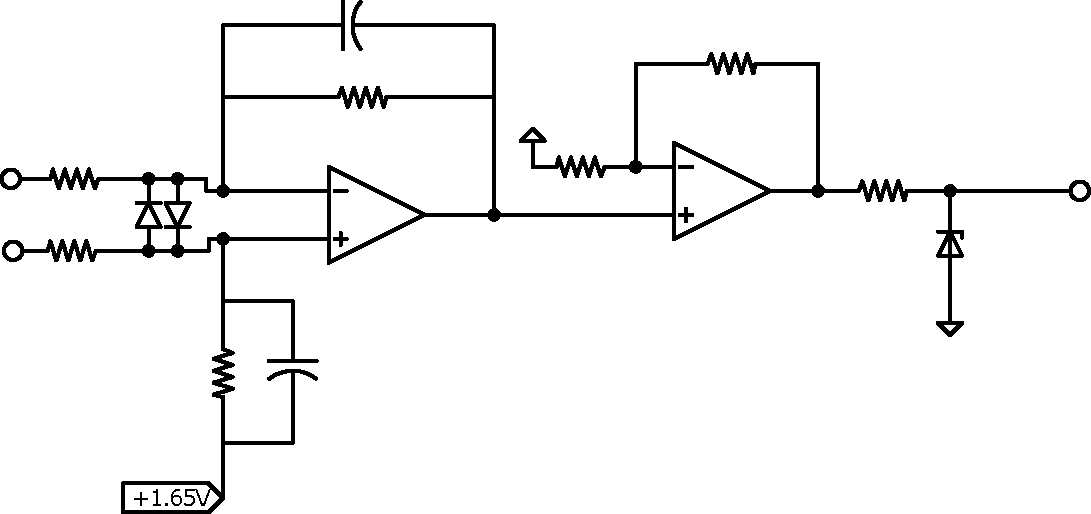
\includegraphics[width=0.8\linewidth]{voltage-sensor}
        \caption{Voltage sensing circuit}
        \label{fig:vsens}
    \end{figure}
	The voltage is sensed using potential dividers. Figure \ref{fig:vsens} shows the voltage sensing circuit. Two such circuits are required in the converter to measure the output voltage and the voltage source voltage. A differential amplifier with pre-tuned gain is used to measure the voltage. The output of differential amplifier is passed through a unity follower before reading by the ADC to overcome any current requirement shortcoming of the previous stage. It is worth noting that the operational amplifiers used in this hardware have a unity gain bandwidth if 3 MHz. A zener diode is used at the output for over voltage protection of the ADC. A reference voltage is manually added to extend the full scale measurement to negative voltages as the ADC is capable of measuring only positive voltages. The overall range of measurement is -120 to +130 V.
	\begin{figure}[h]
        \centering
        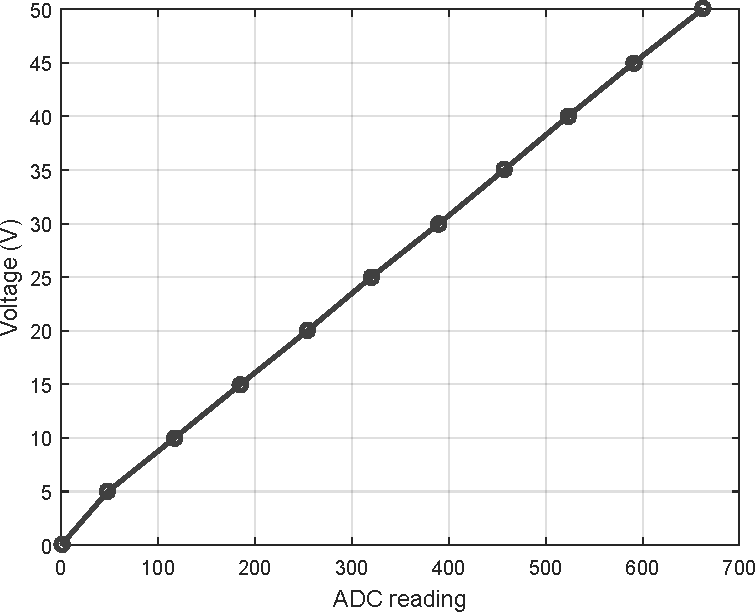
\includegraphics[width=0.6\linewidth]{voltage2_cal}
        \caption{Voltage sensor calibration}
        \label{fig:voltage2-cal}
    \end{figure}
	The calibration of the voltage sensor has been carried out by observing the ADC values as read by the DSP while the input voltage is varied from 0 to 50V in steps of 5V. A linearly regressed line is fitted through these points and the values of slope and the intercept are then used to calculate the actual voltage from the ADC values. Figure \ref{fig:voltage2-cal} shows the calibration curve for the voltage sensors. The Y-axis represents the voltage and X-axis represents the ADC readings.
	
	A hardware RC filter and a software averaging filter is required in this application due to very small gain requirements because of the large sensing ranges.
	
\subsection{Current Sensors}
    Various off-the-shelf current sensors have been tested for range, output voltage and frequency response before designing a shunt resistor based current sensing  circuits. Each sensor is tested for range by varying the amplitude of a square wave current signal. For testing the response time, the frequency of this signal is gradually increased till the rise time is about $1/5^\text{th}$ of the time period. Table \ref{tab:current-sensor} summarises the observations of these experiments.
	\begin{table}[h]
	\centering
		\begin{tabular}{| l | p{3cm} | p{4cm} | p{4cm} |} \hline
			\textbf{Sensor} & \textbf{Rating} & \textbf{Observations} & \textbf{Comments}\\ \hline
			HLSR 16P & \parbox[t]{3cm}{Voltage = 5V \\ Current = $\pm$40A \\ BW = 400kHz \vspace{1.5mm}} & Low sensed voltage & \parbox[t]{4cm}{$\text{Range}_\text{req}\ll\text{Range}_\text{rated}$ \\ Distortion above 20kHz} \\ \hline
			LA 55P & \parbox[t]{3cm}{Voltage = $\pm$15V \\ Current = $\pm$50A\\BW = 200kHz \vspace{1.5mm}} & Low sensed voltage & \parbox[t]{4cm}{$\text{Range}_\text{req} \ll \text{Range}_\text{rated}$ \\ Distortion above 10kHz} \\ \hline
			ACS 712 & \parbox[t]{3cm}{Voltage = 8V \\ Current = 100A\\BW = 80kHz \vspace{1.5mm}} & High rise time & Low bandwidth \\ \hline
			Shunt resistance & \parbox[t]{3cm}{Voltage = $\pm$5V \\ Current = $\pm$30A\\BW = 3MHz \vspace{1.5mm}} & Low rise time & \parbox[t]{4cm}{Adjustable gain and BW} \\ \hline
		\end{tabular}
		\caption{Current sensor testing}
		\label{tab:current-sensor}
	\end{table}
    \begin{figure}[h]
        \centering
        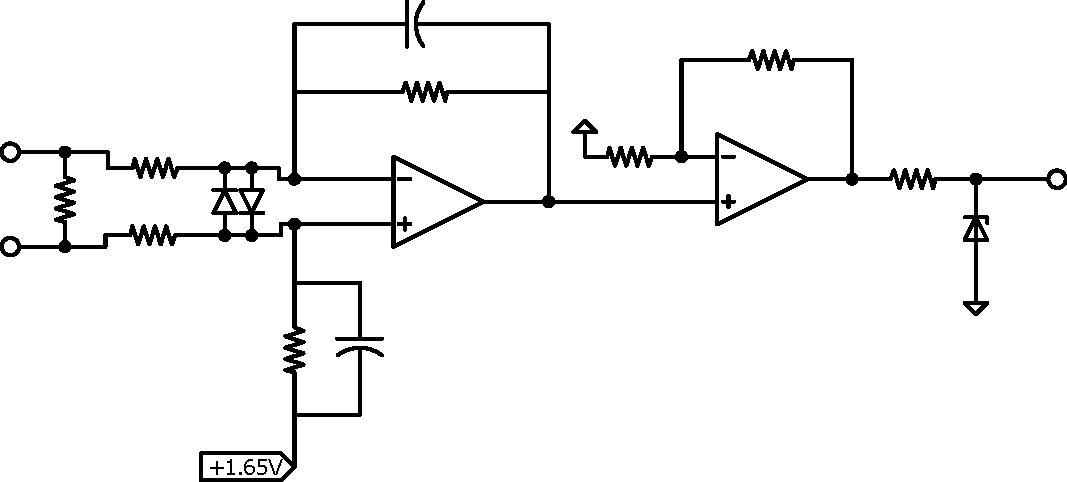
\includegraphics[width=0.8\linewidth]{current-sensor}
        \caption{Current sensing circuit}
        \label{fig:isens}
    \end{figure}
    The voltage drop across a shunt resistor of 0.1 $\Omega$ and 20 W is used to measure the current. Figure \ref{fig:isens} shows the current measurement circuit. The voltage across shunt resistor is fed to differential amplifier circuit to increase the gain. This is then fed to a unity follower. The output protection and bias arrangements are same as the voltage sensor. Three such circuits are required to measure the currents in both inductors and the load current The range of current measurement achieved is -15 to +20 A.
	\begin{figure}[h]
        \centering
        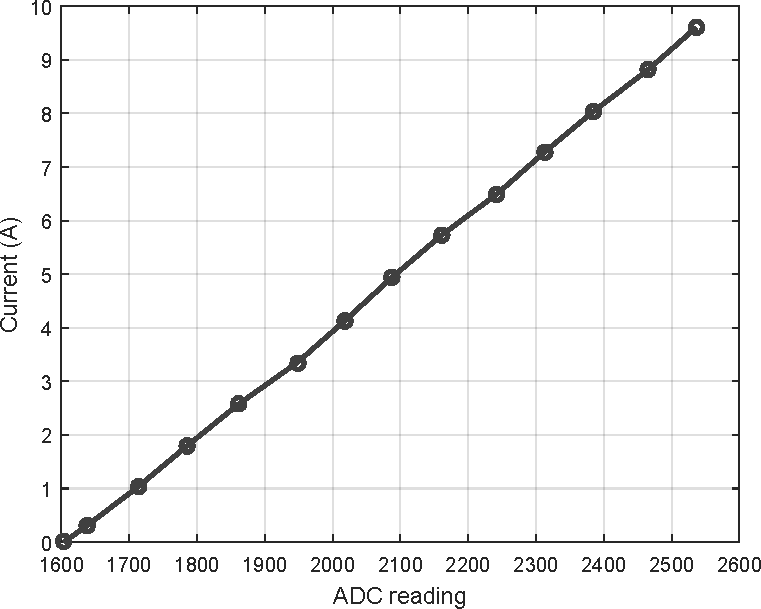
\includegraphics[width=0.6\linewidth]{current2_cal}
        \caption{Current sensor calibration}
        \label{fig:current-cal}
    \end{figure}
	The calibration of current sensor has been carried out via the same procedure as the voltage sensor. The current is varied from 0 to 10A in small steps, then a linear regression curve is fitted through this data. The values of slope and the intercept are then used to obtain the current reading from the ADC values. Figure \ref{fig:current-cal} shows the calibration curve for the current sensor. The Y-axis represents the current values while the X-axis represents the ADC values. No filtering is employed in the current sensor to preserve the small response times.

\section{Power Electronic Switches}
	Initially, every part of the hardware was designed and components were chosen from electronic components available in the market. The details of this MOSFET-based design are given in appendix \ref{app:mosfet-based}. However, considering time constraint and reliability of operation, the power electronic switches along with driver are sourced as ready to use IGBT modules/stacks from Semikron. Following section describe these in brief.
	\begin{figure}[h]
        \centering
        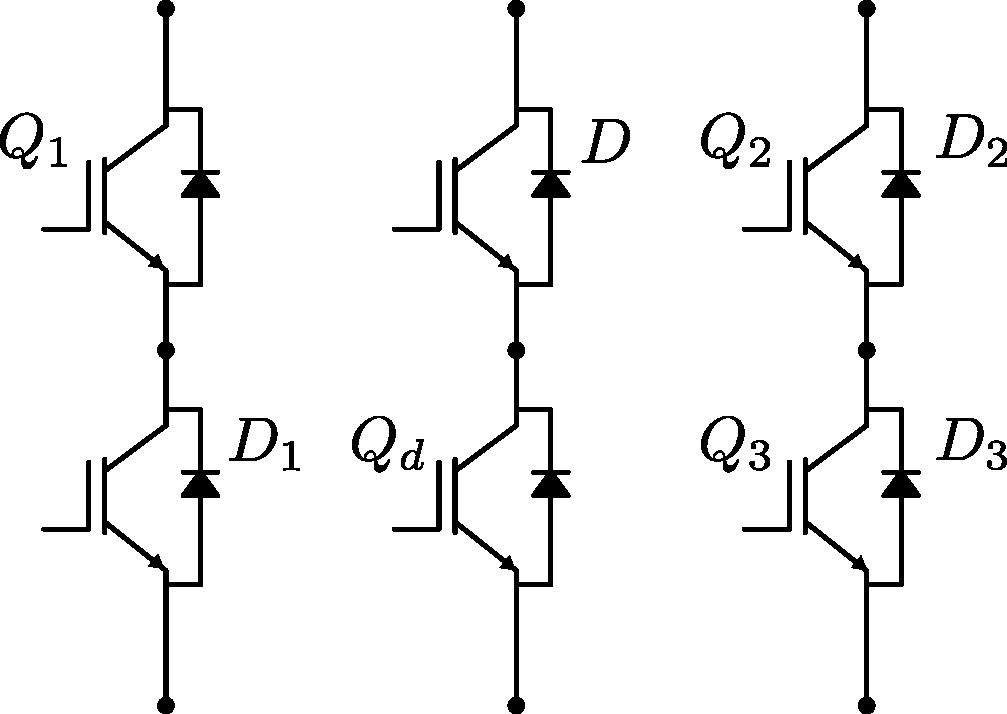
\includegraphics[width=0.4\textwidth]{igbt}
        \caption{IGBT module configuration}
        \label{fig:igbt}
    \end{figure}
    Figure \ref{fig:igbt} is representation of the IGBT modules used for switching in the proposed converter topology. The first module is used as the current controlled single quadrant converter with devices $Q_1$ and $D_1$ as marked. The switches $Q_2$ and $Q_3$ from the last module are acting as voltage controlled two quadrant converter. The ignition control scheme is realised using the second module with devices $Q_d$ and $D$. The diodes $D_1$ and $D$ are the body diodes of the IGBTs which always remain OFF during the entire operation. The rating of the switches in the ignition control module is 1200 V, 88 A, 20 kHz while that of the two converter modules is 600 V, 150 A, 500 kHz.
	\begin{table}[h]
		\centering
		\begin{tabular}{| l | l | p{4cm} |} \hline
			\textbf{Module} & \textbf{IGBT} & \textbf{Rating} \\ \hline
			1, 3 & SKM145GB066D & \parbox[t]{4cm}{$V_{CE}$=600V \\ $I_{C}$=190A \\ $I_D$=150A \\ $t_r$=52ns \\ $t_f$=45ns \\ $t_{d(ON)}$=150ns \\ $t_{d(OFF)}$=450ns} \vspace{-1mm} \\ \hline
			2 & SKM75GB12T4 & \parbox[t]{4cm}{$V_{CE}$=1200V \\ $I_{C}$=115A \\ $I_D$=97A \\ $t_r$=39ns \\ $t_f$=66ns \\ $t_{d(ON)}$=150ns \\ $t_{d(OFF)}$=370ns} \vspace{-1mm} \\ \hline
		\end{tabular}
		\caption{IGBT module ratings}
		\label{tab:igbt}
	\end{table}

	\section{DSP Board}
	\begin{table}[h]
	\begin{tabular}{|l|l|l|l|} \hline
	\textbf{Function} & \textbf{Number of units} & \textbf{Rating} & \textbf{Utility} \\ \hline
	CPU & 1 & 90 MIPS & Executing control laws \\ \hline
	CLA & 1 & 90 MIPS & Sampling and filtering ADC inputs \\ \hline
	ADC & 16 & 0 to 3.3 V, 3.46 MSPS & 5 channels for sensing\\ \hline
	ePWM & 16 & $\text{V}_\text{L}$ = 0V, $\text{V}_\text{L}$ = 3.3 V & 6 channels for IGBTs\\ \hline
	\end{tabular}
	\caption{DSP specifications}
	\label{tab:dsp}
	\end{table}
	
    The F28069 Piccolo series processor operates at 90 MHz system clock. Table \ref{tab:dsp} summarises the important specifications of this DSP. Six ePWM channels and five ADC channels from this processor are utilised in the normal operation of the pulsed power supply. The ADC sampling and controller execution frequencies are set to 50 kHz.

    Figure \ref{fig:interfacing} shows the interfacing circuit for switching signals from the ePWM channel output to the gate driver input of the IGBT modules. A voltage buffer is used to change the voltage level of switching signals from 3.3 V to 15 V as per the requirements of the gate driver circuit. A unity follower is used to mitigate voltage drop issues due to the current requirements of the gate driver.

	\begin{figure}[h]
        \centering
        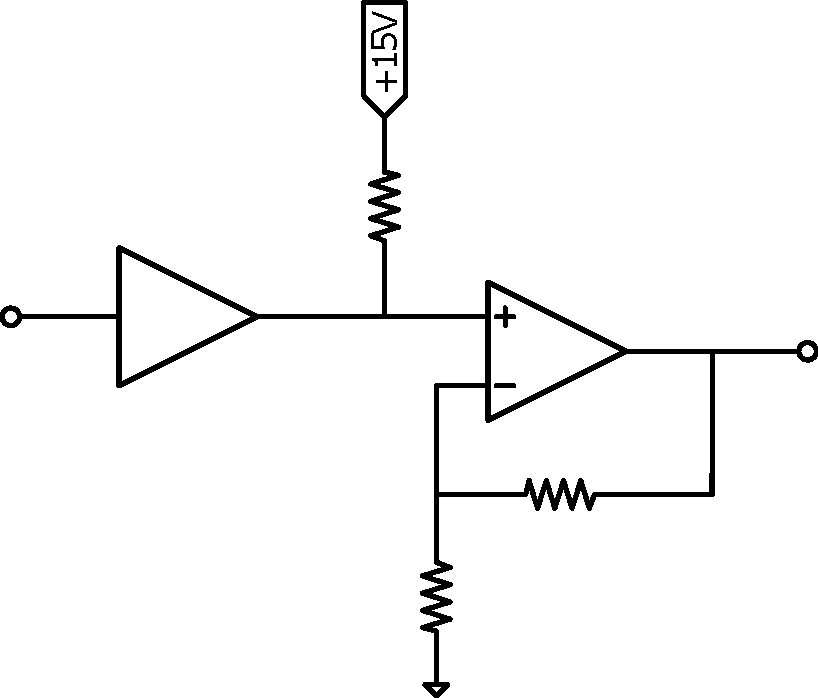
\includegraphics[width=0.4\textwidth]{interfacing}
        \caption{DSP interfacing circuit}
        \label{fig:interfacing}
    \end{figure}
	\begin{figure}[h]
        \centering
        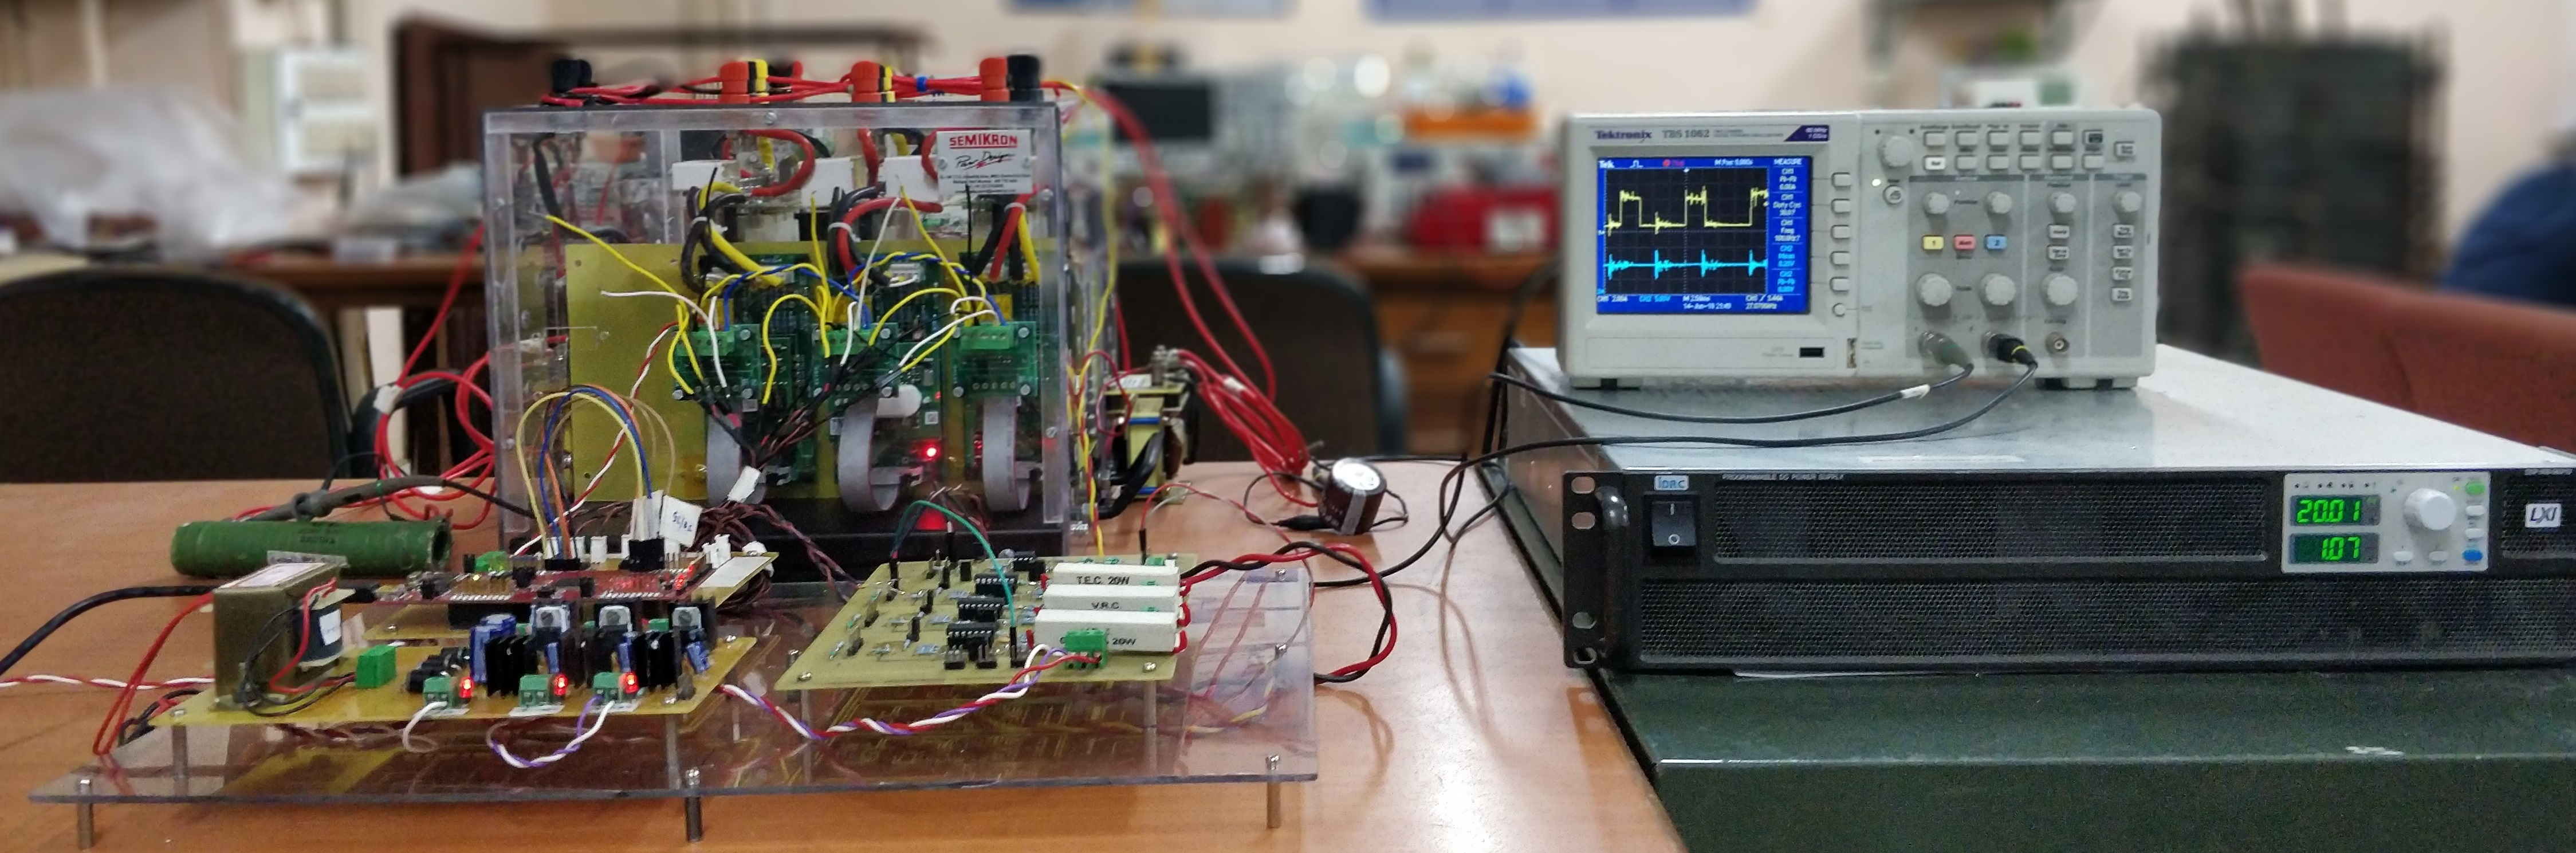
\includegraphics[width=0.8\textwidth]{setup}
        \caption{Complete experimental setup of pulsed power supply}
        \label{fig:setup}
    \end{figure}
    \begin{figure}[h]
        \centering
        \includegraphics[width=0.7\textwidth,angle=90]{interfacing-image}
        \caption{DSP interfacing hardware}
        \label{fig:interfacing-image}
    \end{figure}

%\Chapter{Results and Discussions}
\Chapter{Results and Conclusions}
\label{chap:results}
    This chapter summarises the results of simulation of entire converter using PID control and current mode control techniques. The experimentation results on the hardware setup are also presented herein.

\section{Simulations}
	The values of components derived in chapter \ref{chap:hardware} are used in a simulation of the converter with 50 kHz switching frequency and 5 kHz machining frequency. Table \ref{tab:sim1-param} enlists the simulation parameters used.
	\begin{comment}
		The voltage and current waveforms across the load when direct duty ratio control is used are shown in figure \ref{fig:1b}. Figure \ref{fig:sim-cmc} shows the load voltage and current waveforms when current mode control is used. The output waveforms thus obtained are in well agreement with the results in \cite{tastekin2009novel}.
		\begin{figure}[H]
			\begin{subfigure}{0.49\textwidth}
				\centering
				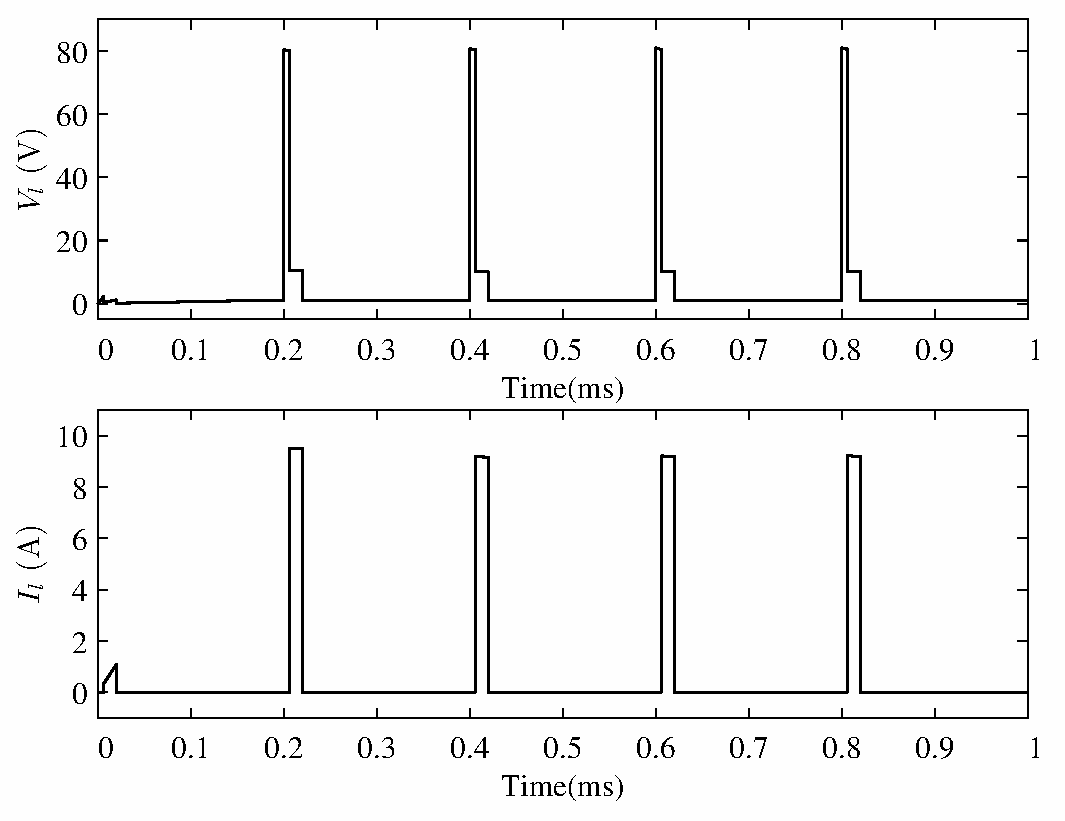
\includegraphics[width=0.95\linewidth]{load_comp}
				\caption{Direct duty ratio control}
				\label{fig:1b}
			\end{subfigure}
			\begin{subfigure}{0.49\textwidth}
				\centering
				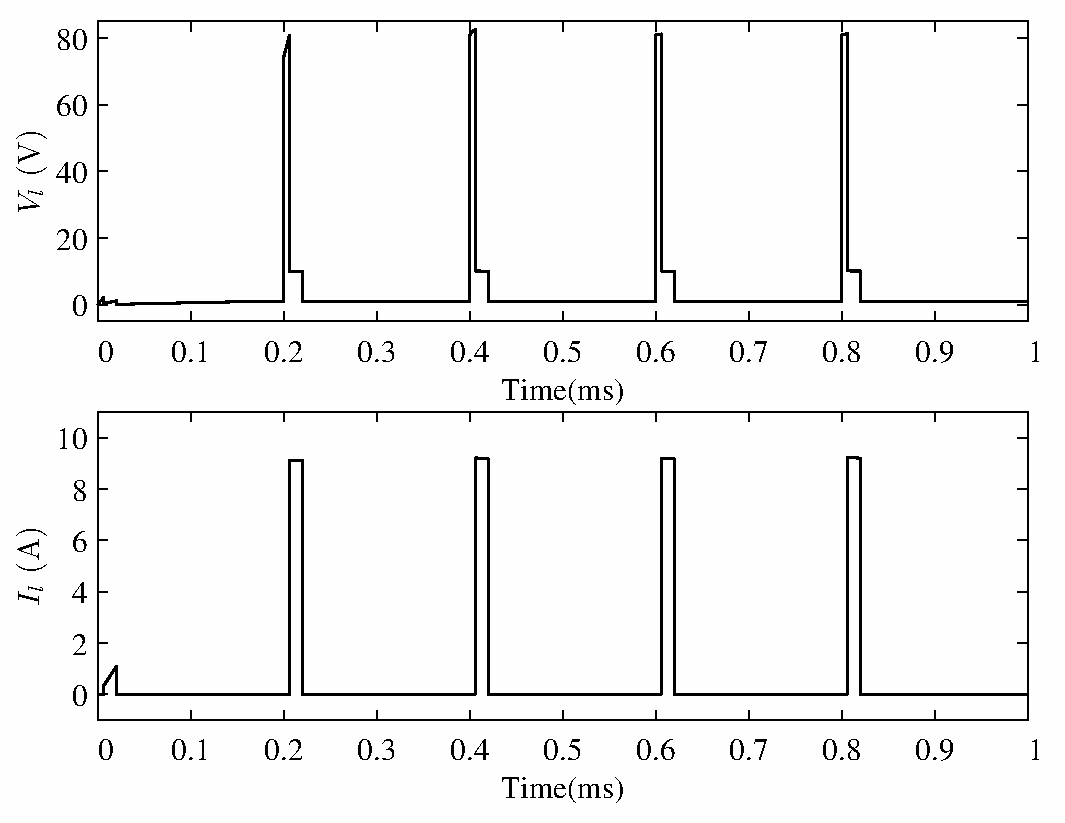
\includegraphics[width=0.95\linewidth]{load_cmc}
				\caption{Current mode control}
				\label{fig:sim-cmc}
			\end{subfigure}
			\caption{Load voltage and current}
		\end{figure}
		Figure \ref{fig:sim-qd} shows the voltage across $Q_d$ and current through $Q_d$ waveforms when direct duty ratio control is used. The maximum voltage across $Q_d$ is $V_{\text{ref}}$ i.e. 80 V and and the maximum current through $Q_d$ is 11 A during the rise time. Figure \ref{fig:sim-d} shows the voltage across $D$ and current through $D$ waveforms when direct duty ratio control is used. The maximum reverse voltage across $D$ is 83 V and the maximum forward current through it is 0.8 A.
		\begin{figure}[H]
			\begin{subfigure}{0.49\textwidth}
				\centering
				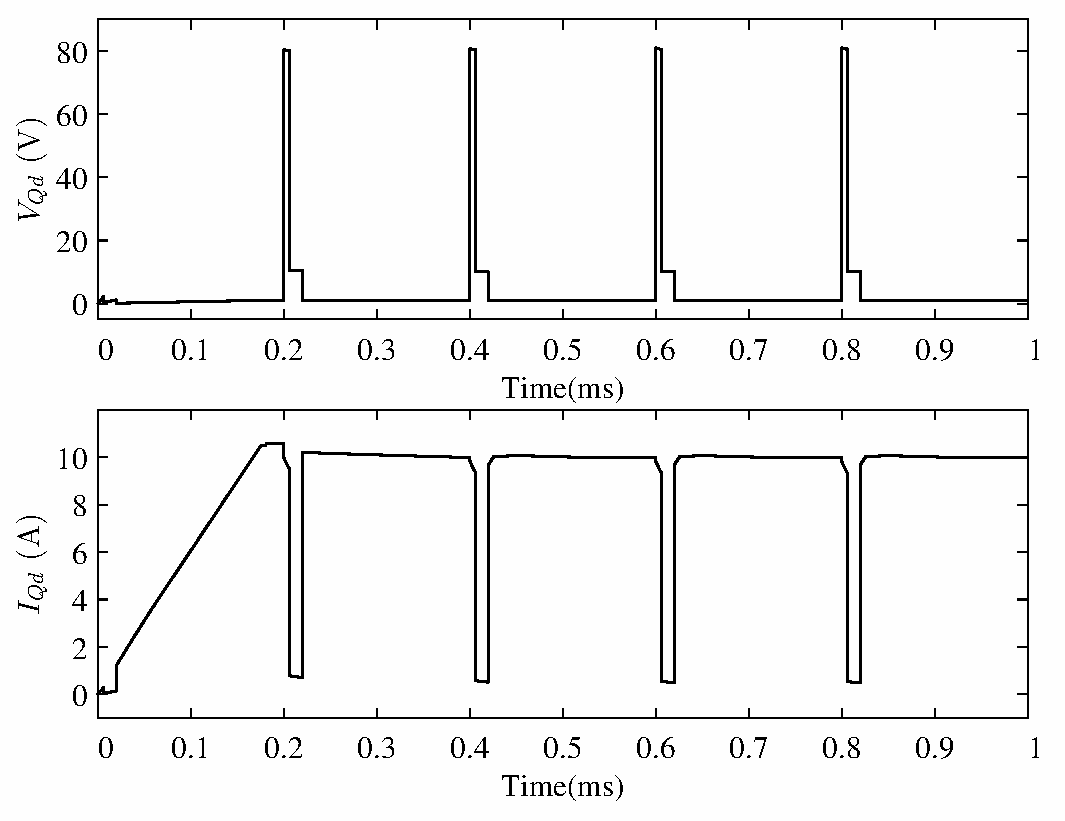
\includegraphics[width=0.95\linewidth]{Qd}
				\caption{Voltage and current of Qd}
				\label{fig:sim-qd}
			\end{subfigure}
			\begin{subfigure}{0.49\textwidth}
				\centering
				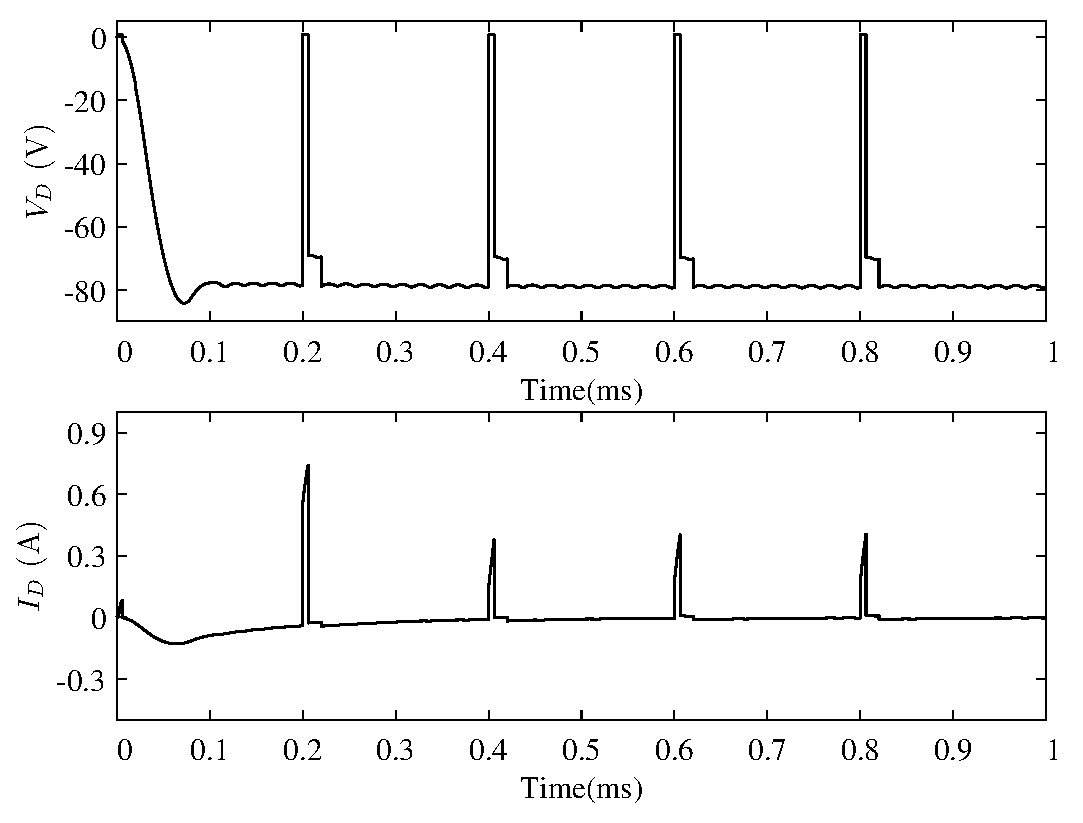
\includegraphics[width=0.95\linewidth]{D}
				\caption{Voltage and current of D}
				\label{fig:sim-d}
			\end{subfigure}
			\caption{Direct duty ratio control: Qd,D}
		\end{figure}
		Figure \ref{fig:sim-q1} shows the voltage across $Q_1$ and current through $Q_1$ waveforms when direct duty ratio control is used. The maximum voltage across $Q_1$ is $V_d$ i.e 110 V and the maximum current through it is 11 A. Figure \ref{fig:sim-d1} shows the voltage across $D_1$ and current through $D_1$ waveforms when direct duty ratio control is used. The maximum reverse voltage across diode $D_1$ is $V_d$ i.e. 110 V and the maximum forward current through it is 11 A.
		\begin{figure}[H]
			\begin{subfigure}{0.49\textwidth}
				\centering
				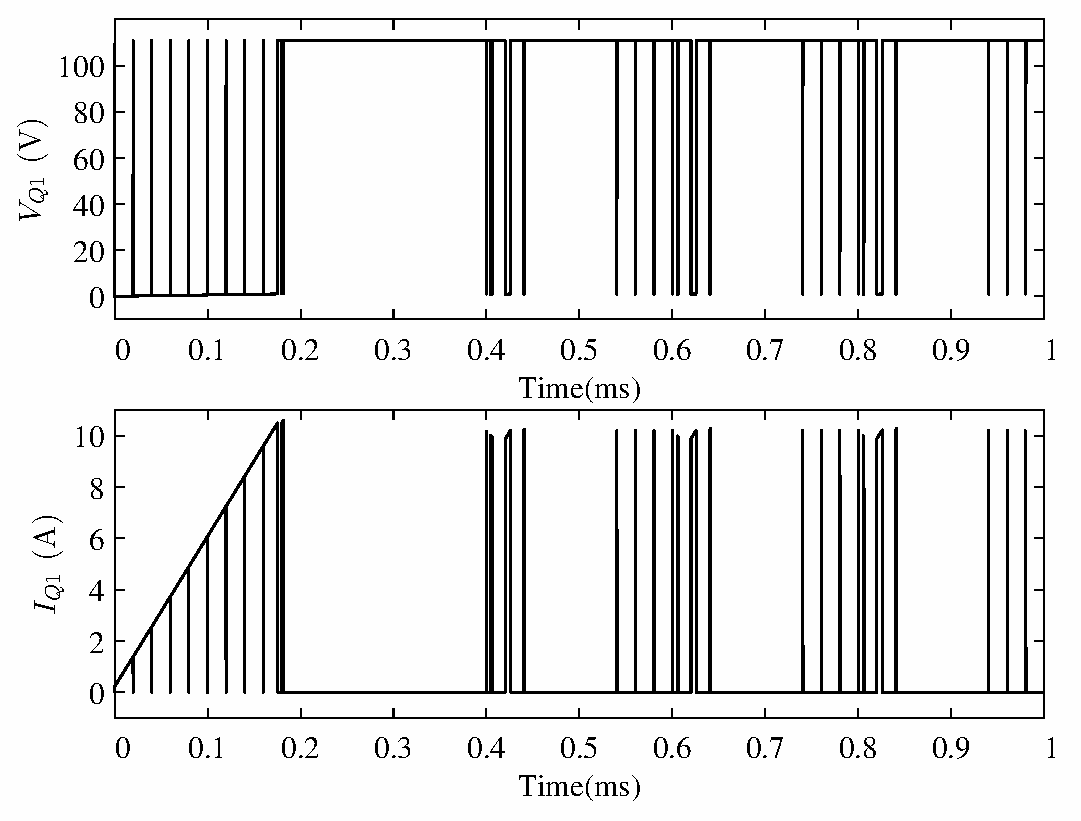
\includegraphics[width=0.95\linewidth]{Q1}
				\caption{Voltage and current of Q1}
				\label{fig:sim-q1}
			\end{subfigure}
			\begin{subfigure}{0.49\textwidth}
				\centering
				\includegraphics[width=0.95\linewidth]{D1}
				\caption{Voltage and current of D1}
				\label{fig:sim-d1}
			\end{subfigure}
			\caption{Direct duty ratio control: Q1,D1}
		\end{figure}
		Figure \ref{fig:sim-q2} shows the voltage across $Q_2$ and current through $Q_2$ waveforms when direct duty ratio control is used. The maximum voltage across $Q_2$ is $V_d$ i.e 110 V and the maximum current through it is 21 A. This maximum occurs during the rise time of the voltage source. Figure \ref{fig:sim-d2} shows the voltage across $D_2$ and current through $D_2$ waveforms when direct duty ratio control is used. The maximum reverse voltage across $D_2$ is $V_d$ i.e. 110 V and the maximum current through it is 4.5 A.
		\begin{figure}[H]
			\begin{subfigure}{0.49\textwidth}
				\centering
				\includegraphics[width=0.95\linewidth]{Q2}
				\caption{Voltage and current of Q2}
				\label{fig:sim-q2}
			\end{subfigure}
			\begin{subfigure}{0.49\textwidth}
				\centering
				\includegraphics[width=0.95\linewidth]{D2}
				\caption{Voltage and current of D2}
				\label{fig:sim-d2}
			\end{subfigure}
			\caption{Direct duty ratio control: Q2,D2}
		\end{figure}
		Figure \ref{fig:sim-q3} shows the voltage across $Q_3$ and current through $Q_3$ waveforms when direct duty ratio control is used. The maximum voltage across $Q_3$ is 110 V and the maximum current through it is 4.5 A. Figure \ref{fig:sim-d3} shows the voltage across $D_3$ and current through $D_3$ waveforms when direct duty ratio control is used. The maximum reverse voltage across $D_3$ is 110 V and the maximum current through it is 21 A.
		\begin{figure}[H]
			\begin{subfigure}{0.49\textwidth}
				\centering
				\includegraphics[width=0.95\linewidth]{Q3}
				\caption{Voltage and current of Q3}
				\label{fig:sim-q3}
			\end{subfigure}
			\begin{subfigure}{0.49\textwidth}
				\centering
				\includegraphics[width=0.95\linewidth]{D3}
				\caption{Voltage and current of D3}
				\label{fig:sim-d3}
			\end{subfigure}
			\caption{Direct duty ratio control: Q3,D3}
		\end{figure}
	\end{comment}
	\begin{table}[H]
		\centering
			\begin{tabular}{|l|l|} \hline
				Current source inductor & 2 mH \\ \hline
				Voltage source inductor & 100 $\mu$H \\ \hline
				Voltage source capacitor & 100 $\mu$F \\ \hline
				Switching frequency & 50 kHz \\ \hline
				Machining frequency & 5 kHz at 10\% duty \\ \hline
				DC link voltage & 110 V \\ \hline
				Current reference & 10 A \\ \hline
				Voltage reference & 80 V \\ \hline
				Load resistance & 1 $\Omega$ \\ \hline
			\end{tabular}
		\caption{Simulation parameters}
		\label{tab:sim1-param}
	\end{table}
\subsection{PI Control}
	\begin{figure}[H]
		\centering
		\includegraphics[width=0.6\textwidth]{results_2mh_pi}
		\caption{Load voltage and current: PI control}
		\label{fig:results_2mh_pi}
	\end{figure}
	Figure \ref{fig:results_2mh_pi} shows the load voltage and the load current when both the converters are controlled by PI controllers. The output waveforms thus obtained are similar to the results in \cite{tastekin2009novel}. The voltage source output is shown in figure \ref{fig:vs_2mh_pi} and the current source output is shown in figure \ref{fig:cs_2mh_pi}. The responses of both the sources are overdamped and their rise times are below 0.5 ms.
	\begin{figure}[H]
		\centering
		\begin{subfigure}{0.49\linewidth}
			\includegraphics[width=\linewidth]{cs_2mh_pi}
			\caption{Voltage source output}
			\label{fig:cs_2mh_pi}
		\end{subfigure}
		\begin{subfigure}{0.49\linewidth}
			\includegraphics[width=\linewidth]{vs_2mh_pi}
			\caption{Current source output}
			\label{fig:vs_2mh_pi}
		\end{subfigure}
		\caption{PI control}
	\end{figure}
	table \ref{tab:power} summarises the observed power consumption during the operation under constant reference as well as pulsed reference for the current source. The majority of the power is lost in $r_L, Q_d, D_1$ as the machining duty for the WEDM process is very low.
	\begin{table}[H]
		\centering
		\begin{tabular}{|c|c|c|} \hline
			\textbf{Component} & \textbf{Power (Const. ref.)} & \textbf{Power (Pulsed ref.)} \\ \hline
			Source & 24.81 W & 11.99 W \\ \hline
			Load & 7.34 W & 7.34 W \\ \hline
			$r_L, Q_d, D_1$ & 16.47 W & 3.82 W \\ \hline
			Other & 1.06 W & 0.83 W \\ \hline
		\end{tabular}
		\caption{Power consumption for pulsed reference scheme}
		\label{tab:power}
	\end{table}

\subsection{Current Mode Control}
	\begin{figure}[H]
		\centering
		\includegraphics[width=0.6\textwidth]{results_2mh_cmc}
		\caption{Load voltage and current: Current mode control}
		\label{fig:results_2mh_cmc}
	\end{figure}
	Figure \ref{fig:results_2mh_cmc} shows the load voltage and the load current when both the converters are controlled via current mode control. While the load voltage and current are similar to the PI controller, the the response of voltage source is underdamped. The settling times of the voltage source is about 1 s while that of the current source is same as the previous. The voltage source output is shown in figure \ref{fig:vs_2mh_cmc} and the current source output is shown in figure \ref{fig:cs_2mh_cmc}.
	\begin{figure}[H]
		\centering
		\begin{subfigure}{0.49\linewidth}
			\includegraphics[width=\linewidth]{cs_2mh_cmc}
			\caption{Voltage source output}
			\label{fig:cs_2mh_cmc}
		\end{subfigure}
		\begin{subfigure}{0.49\linewidth}
			\includegraphics[width=\linewidth]{vs_2mh_cmc}
			\caption{Current source output}
			\label{fig:vs_2mh_cmc}
		\end{subfigure}
		\caption{Current mode control}
	\end{figure}
\subsection{Compensator Based Control}
	\begin{figure}[H]
		\centering
		\includegraphics[width=0.6\textwidth]{results_2mh_comp}
		\caption{Load voltage and current: Compensators}
		\label{fig:results_2mh_comp}
	\end{figure}
	Figure \ref{fig:results_2mh_pi} shows the load voltage and the load current when both the converters are controlled by lead-lag compensators. The voltage source output is shown in figure \ref{fig:vs_2mh_comp} and the current source output is shown in figure \ref{fig:cs_2mh_comp}. The current source is underdamped while the voltage source is overdamped with a significant settling time of 4 s. Several notches are present in the current source output during the pre-breakdown stages of the machining. However, there is no observable deviation from the expected load current and voltage. These are also observable in the hardware experiments and the possible causes are summarised later in this chapter.
	\begin{figure}[H]
		\centering
		\begin{subfigure}{0.49\linewidth}
			\includegraphics[width=\linewidth]{cs_2mh_comp}
			\caption{Voltage source output}
			\label{fig:cs_2mh_comp}
		\end{subfigure}
		\begin{subfigure}{0.49\linewidth}
			\includegraphics[width=\linewidth]{vs_2mh_comp}
			\caption{Current source output}
			\label{fig:vs_2mh_comp}
		\end{subfigure}
		\caption{Compensator based control}
	\end{figure}
	
\section{Hardware Experiments}
	\begin{figure}[h]
		\centering
		\begin{subfigure}{0.49\linewidth}
			\includegraphics[width=\linewidth]{hardware-expt1}
			\caption{Operation with fixed resistance}
			\label{fig:hardware-expt1}
		\end{subfigure}
		\begin{subfigure}{0.49\linewidth}
			\includegraphics[width=\linewidth]{hardware-expt2}
			\caption{Operation with load switch}
			\label{fig:hardware-expt2}
		\end{subfigure}
		\caption{Hardware experiments}
	\end{figure}
	Table \ref{tab:hardware-param} summarises the specifications of the hardware setup which is used for experimentation. The operation of converter has been tested with a fixed load resistance as well as the combination of a resistance and switch. Figure \ref{fig:hardware-expt1} shows the load configuration for the first experiment where the current source is tested for disturbances. Another experiment has been carried out to test the converter in sparking like conditions. The load resistance is connected through the switch as shown in figure \ref{fig:hardware-expt2}.
	\begin{table}[h]
		\centering
			\begin{tabular}{|l|l|} \hline
				Current source inductor & 100$\mu$H \\ \hline
				Voltage source inductor & 2 mH \\ \hline
				Voltage source capacitor & 1000 $\mu$F \\ \hline
				Switching frequency & 50 kHz \\ \hline
				Machining frequency & 1 kHz at 50\% duty \\ \hline
				DC link voltage & 20 V \\ \hline
				Current reference & 4 A \\ \hline
				Voltage reference & 15 V \\ \hline
				Load resistance & 1 $\Omega$ \\ \hline
			\end{tabular}
		\caption{Experimental hardware specifications}
		\label{tab:hardware-param}
	\end{table}
	
\subsection{Operation With Fixed Load Resistance}
    The hardware setup developed in chapter \ref{chap:hardware} is used for initial experimentation with the converters. A load of 1 $\Omega$ is connected to the current controlled single quadrant converter. The ignition control switch is connected in parallel to this load to test for the response to disturbance to variable structure of the current source load. The current through the load resistor and the output voltage of the voltage controlled two quadrant converter is measured.
    \begin{figure}[H]
	    \begin{subfigure}{0.49\textwidth}
    		\centering
    		\includegraphics[width=0.95\linewidth]{switching-results}
    		\caption{Current Source switching test}
    		\label{fig:sw-results}
		\end{subfigure}
	    \begin{subfigure}{0.49\textwidth}
        	\centering
        	\includegraphics[width=0.95\linewidth]{transient}
    		\caption{Transient performance of current source}
    		\label{fig:transient}
		\end{subfigure}
		\caption{Current source performance under switching}
	\end{figure}
	Figure \ref{fig:sw-results} shows the current through the load resistor when ignition switch is operated at 1 kHz and the switching frequency of the converter itself is 100 kHz. The DC link voltage for this experiment is kept at 20 V. Voltage spikes corresponding to the ringing are observed in the current waveform. The transient performance of the current source under these conditions is shown in figure \ref{fig:transient}. It takes about 100 $\mu$s time for the current source to return to its normal operation after ignition switch is opened.
	\begin{comment}
	\begin{figure}[H]
		\centering
		\includegraphics[width=0.6\textwidth]{vsource-result}
		\caption{Voltage Source steady state performance}
		\label{fig:vsource-result}
	\end{figure}
	The steady state no load performance of the voltage source is shown in figure \ref{fig:vsource-result}. The conditions for this observations were same as the above.
	\end{comment}
	
\subsection{Operation With Load Switch}
	Figure \ref{fig:results} depicts the observed waveforms during complete operation of the converter. The ignition switch, which controls the machining duty is operated at 1kHz on 50\% duty while the switching frequencies of both the individual converters during this experiment is 50kHz. The load is a 1$\Omega$ resistance with a switch operating at 1kHz on 30\% duty to replicate the sparking phenomenon. The switching signals for the ignition switch and the load switch are on the top for comparison. The voltage and current are observed across the load terminals. The voltage across the diode D is also observed.
	
	When the ignition switch is opened, the diode D is forward biased and the voltage source output of 15V is reflected at the load terminals until the load switch is closed. Once the load switch is closed (representative of ignition of spark), the current is diverted through the load of 1$\Omega$ and the diode D is turned OFF. Hence, the voltage observed at the load terminals is the IR drop. When the ignition switch is closed, the current is diverted through the ignition switch which offers the lowest resistance path for the current flow and the voltage observed across the load terminals is the ON time voltage drop of the ignition switch. The current is allowed through the load only when the load switch is closed and its value during this period is the set reference of the current source.

	\begin{figure}[H]
		\centering
		\includegraphics[width=\textwidth]{results}
		\caption{Results}
		\label{fig:results}
	\end{figure}

	\begin{comment}
		\begin{figure}[H]
			\centering
			\includegraphics[width=0.6\textwidth]{results2}
			\caption{Hardware results for operation under switched R load}
			\label{fig:results2}
		\end{figure}
		The entire operation of the proposed converter relies on the fact that the voltage source output will appear across the spark gap terminals when the diode D is ON. To verify this, the above experiment has been run at the machining frequency of 100Hz to observer the behaviour of the converter under larger disturbance. It is observed that the load voltage follows the voltage source output when the D is ON. This is shown in figure \ref{fig:results2}.
	\end{comment}
	
	\begin{figure}[H]
		\centering
		\begin{subfigure}{0.49\textwidth}	
			\includegraphics[width=\linewidth]{l1current}
			\caption{Current source output}
			\label{fig:l1current}
		\end{subfigure}
		\begin{subfigure}{0.49\textwidth}
			\includegraphics[width=\linewidth]{c2voltage}
			\caption{Voltage source output}
			\label{fig:c2voltage}
		\end{subfigure}
		\caption{Individual converter performance under switched R load}
	\end{figure}
	
	Figure \ref{fig:c2voltage} shows the voltage source output i.e. the voltage across the voltage source capacitor. This voltage is equal to the reference voltage of 15 V. The current source output is shown in .For the current source, the inductor current is the output which is shown in figure \ref{fig:l1current}. This current is deviates from the expected output which should be a constant line of 4 A. The table \ref{tab:l1current} summarises the operation of the current source as observed in the second experiment.
	\begin{table}[H]
		\centering
		\begin{tabular}{|l|l|l|l|} \hline
		\textbf{Ref. in figure} & \textbf{Stage} & \textbf{Observation} & \textbf{Comments} \\ \hline
		1 & Sparking & $I_{L_1} \approx I_{ref}$ with some transients & Expected \\ \hline
		2 & Dead time & $I_{L_1} > I_{ref}$ & Not expected \\ \hline
		3 & Pre-breakdown & $I_{L_1} \approx 0$ A & Not expected \\ \hline
		\end{tabular} 
		\caption{Current source observations}
		\label{tab:l1current}
	\end{table}
	The load observed by the current source changes with the discharge stage, hence it is a Variable Structure System (VSS). The current source is tuned for fixed 1 $\Omega$ resistance load, therefore the current observed during the sparking stage is as expected. However, during the dead time, load seen by the current source is a short circuit condition. This condition offers least resistance path for the current causing the current to increase above the set reference. The linear controllers may not perform optimally for variable structured systems.
	
	The current dip during the pre-breakdown stage is result of low inductor value in the current source. This observation has been verified via simulations and the dip gets reduced for higher inductor values. This observation is consistent across the current mode control and the compensator based control. The energy stored in the inductor from the dead time is $1/2LI^2 = 0.125 mJ$, when the ignition switch is opened this energy is transferred to the capacitor via the decoupling diode. The voltage at the capacitor terminals increases according to the energy balance equation for this transfer.
	\begin{align*}
		\therefore \dfrac{1}{2}L(I_1^2 - I_2^2) &= \dfrac{1}{2}C(V_2^2 - V_1^2) \\
		\dfrac{1}{2}100\times 10^{-6}(5^2 - 0) &= \dfrac{1}{2}1000\times10^{-6}(V_2^2 - 15^2) \\
		V_2 &= 15.08 V
	\end{align*}
	Because the change in capacitor voltage is very small it is not observable from the output voltage waveforms. The entire energy stored in the inductor from the dead time is transferred to the voltage source capacitance causing only a small change in its voltage. As a result, the inductor current goes to zero.
	
	This means that the original assumption of current and voltage sources operating independently is not entirely true. The assumption is valid only when the inductor is large enough to cause a voltage disturbance which detectable and corrected by the voltage source. In the simulation results with a current source inductor of 2 mH, these voltage bumps are observed and handled by the voltage source. Thus, the current dips are lesser in the magnitude. Thus, the less inductor size and linear controller on VSS together cause the observed output current waveform. One possible solution to this issue is decreasing the voltage source capacitor as it is overrated for the present experimentation. The sliding mode controller can be used to maintain almost similar performance across all the VSS states.
\section{Conclusions}
\label{conclusions}
	A pulsed power supply has been developed for Wire Electric Discharge Machining application based on the original topology proposed by \citet{tastekin2009novel}. The this topology deviates from the standard DC-DC converter topologies leading to reduction in the damping factor as observed in the frequency responses in figure \ref{fig:uncomp-vs}. Moreover, due to these modifications standard ripple based sizing criteria is not adequate. Hence, the the appropriate values of L and C have inferred from the trajectories of the poles, which has been verified via the hardware setup.

	The ON state losses via the ignition switch dissipate power for about 70\% to 90\% of the time due to the low machining period requirement of the EDM process. These losses are reduced by lowering the current source reference during the dead time. The time averaging leads to only and approximate model of the converters. Hence, non linear model and sliding mode control has been designed and simulated for individual current and voltage sources each.
	
	The Semikron IGBT modules and the passive components have been assembled according to the topology mentioned in figure \ref{fig:working-3}.  PI controllers have implemented on a TI F28069 DSP board. The IGBTs are interfaced to the DSP via a buffer circuit. The operation of complete converter has been tested for DC link voltage of 20 to 50V at machining frequency of 1kHz.

	The current and voltage sensors with required range and bandwidth are not readily available. Hence, these sensors have been made using shunt resistance and potential dividers along with OP-AMP based conditioning circuits. The biases and slopes of the sensor response have been experimentally found out for their calibration.
	
	The voltage source used in the hardware is found to be working satisfactory but its output capacitor is overrated for the experimental conditions. The current source output had three distinct regions: (a) constant 4 A current region, (b) constant 5 A current region, and (c) zero current region. The possible reasons for these discrepancies have been identified which led to the conclusion that the current and voltage sources operate independently only for a sufficiently large current source inductor.

\section{Future Work}
\begin{itemize}
\item The sensors used in this work are based on resistances with 5\% tolerance band resulting in poor accuracy of the measurements. Moreover, the low power rating of these resistances limit operation to lower currents. This could be improved by using high precision measurement resistances.
\item The unexpected behaviour of the current source inductor as described in table \ref{tab:l1current} can be addressed by reducing the voltage source capacitor. Also, appropriate resizing of inductors and capacitors may be required for desired operation of the converter with an actual spark-gap load.
\item The pulsed reference scheme and sliding mode controller are illustrated with simulations only. The hardware implementation of the sliding mode controller can partially improve the current source inductor behaviour due its nonlinear nature.
\item The hardware experimentation has been done at reduced voltage and current levels. These levels have to be increased while experimenting with the spark-gap test cell.
\end{itemize}
	
\section{Publications}
The following paper is submitted based on the work done in this project.\\
M. Kane, \textbf{A. Khadse}, H. Bahirat, S. Kulkarni, ``Design and Control of Pulsed Voltage Supply for Electric Discharge Machining,'' in \textit{IEEE International Conference on Power Electronics, Drives and Energy Systems}, 2018 (Submitted)
%%\Chapter{Summary and Conclusions}
\section{Conclusions}
\label{conclusions}
	A pulsed power supply was developed for Wire Electric Discharge Machining application based on the original topology proposed by \citet{tastekin2009novel}. The this topology deviates from the standard DC-DC converter topologies leading to reduction in the damping factor as observed in the frequency responses in \Figref{fig:uncomp-vs}. Moreover, due to these modifications standard ripple based sizing criteria is not adequate. Hence, the the appropriate values of L and C were inferred from the trajectories of the poles, which were verified via the hardware setup.

	The ON state losses via the ignition switch dissipate power for about 70\% to 90\% of the time due to the low machining period requirement of the EDM process. These losses were reduced by lowering the current source reference during the dead time. The time averaging leads to only and approximate model of the converters. Hence, non linear model and sliding mode control was designed and simulated for individual current and voltage sources each.
	
	The Semikron IGBT modules and the passive components were assembled according to the topology mentioned in \Figref{fig:working-3}.  PI controllers were implemented on a TI F28069 DSP board. The IGBTs were driven by were interfaced to the DSP via a buffer circuit. The operation of complete converter was tested for DC link voltage of 20 to 50V at machining frequency of 1kHz.

	The current and voltage sensors with required range and bandwidth were not readily available. Hence, these sensors were made using shunt resistance and potential dividers along with OP-AMP based conditioning circuits. The biases and slopes of the sensor response were experimentally found out for their calibration.
	
	The voltage source used in the hardware was found to be working satisfactory but its output capacitor was overrated for the experimental conditions. The current source output had three distinct regions: (a) constant 4 A current region, (b) constant 5 A current region, and (c) zero current region. The possible reasons for these discrepancies were identified which led to the conclusion that the current and voltage sources operate independently only for a sufficiently large current source inductor.
 
\begin{comment}
    The aim of this project is to facilitate investigations and thereby the development of contemporary process for Si-wafer manufacturing. Each of the previous chapters dealt with a specific sub-problem towards this larger goal. In this concluding chapter, the findings of the work accomplished till date are summarised and their contribution to the entire WEDM process is chalked out.
    
%\section{Design}
\subsection{Design}
    The design procedure for pulsed power supply for the WEDM process as discussed in \autoref{chap:psdesign} and \autoref{chap:hardware} is different form that of standard converters. Due importance was was given to the spark load application resulting in elimination of the capacitor form current source and the resistor from the voltage source. The sizing criteria presented was also found to be working as per the initial experimentation carried.
    
    This avenue will help in fabricating power supplies of semiconductor loads in WEDM processes. The design methodology followed tackles the issue of restricted discrete setting ranges based on a steel grade standard of conventional WEDM equipment.

%\section{Modelling and Control}
\subsection{Modelling and Control}
    The \autoref{chap:modelling} and \autoref{chap:lincontrol} present the basic linear control techniques of PID control, compensator based control, and current mode control. The PID control was implemented on the hardware and used for the experimentation. The above techniques were also simulated and the results were in good agreement with the literature.
    
    This contributes a tried and tested method of PID control for the modified application of the converters for EDM application. Also, several alternatives are investigated which can serve the same purpose, the only constraint being the computation capability of the processor.

%\section{Hardware}
\subsection{Hardware}
    The \autoref{chap:hardware} described the fabrication details of the hardware setup developed. Several issues in sensing circuits were addressed before proposing the final voltage and control circuits. These in situ sensors were tested before being used in the main converter. The power electronic circuit was a pre-assembled IGBT module arrangement with gate drivers. However, the auxiliary circuitry required to drive these switches was designed and tested specifically for the specific processor and drivers.
    
    This work outlines the general requirements and procedure for assembling a power supply unit. The design presented for high frequency current and voltage sensors is of peculiar importance to manufacturing processes as it indirectly helps pacing up the operation.

%\section{Improvement}
\subsection{Improvements}
    The nonlinear control technique of sliding mode control is reviewed in \autoref{chap:nonlinear}. An implementation of this controller was simulated. The steady state error was also addressed in this regard. 
    
    Non linear control techniques overcome the problem of operation in a small neighbourhood of the equilibrium point which is inherent to the linear controllers. Thus, this method can improve the dynamic ranges of the individual current and the voltage sources. This will be of utility in investigation of other unconventional loads for the WEDM process.
\end{comment}

\section{Publications}
The following paper is submitted based on the work done in this project.\\
M. Kane, \textbf{A. Khadse}, H. Bahirat, S. Kulkarni, ``Design and Control of Pulsed Voltage Supply for Electric Discharge Machining,'' in \textit{IEEE International Conference on Power Electronics, Drives and Energy Systems}, 2018 (Submitted)

%****************************************************************
%                         Appendices                           
%****************************************************************
%% Additional, supporting material, such as codes, derivations, etc., can be placed in the appendix
\appendix
%%============================= appendix.tex ====================================
\Chapter{Time Averaging Modelling Technique}
\label{app:modelling}
	The large signal representation of voltage source in figure \ref{fig:working-4} as derived in equation \eqref{eq:mod14}
	\begin{align*}
		\begin{split}
			\dot{x} &= [dA_1+(1-d)A_2]x + [dB_1 + (1-d)B_2]V_d\\
			V_o &= [dC_1+(1-d)C_2]x
		\end{split}
	\end{align*}

	Introducing small perturbations in $x$, $V_o$ and $d$ as
	\begin{equation}
		\begin{split}
			x &= X + \hat{x}\\
			v_o &= V_o + \hat{v_o}\\
			d &= D + \hat{d}
		\end{split}
		\label{eq:mod15}
	\end{equation} 
	Since the transfer function is to be determined between $\hat{v_o}$ and $\hat{d}$, perturbations in $v_d$ are assumed to be zero for simplicity, therefore
	\begin{equation}
		v_d = V_d
		\label{eq:mod16}
	\end{equation}
	Using the fact that at steady state $\dot{X} = 0$ and the equations \eqref{eq:mod15} in equation \eqref{eq:mod14}
	\begin{equation}
		\dot{\hat{x}} = AX + BV_d + A\hat{x} + [(A_1-A_2)X+(B_1-B_2)V_d]\hat{d} + \text{terms with products of $\hat{x}$ and $\hat{d}$ (neglected)} 
		\label{eq:mod17}
	\end{equation}
	where
	\begin{align}
		A &= A_1D+A_2(1-D)\\
		B &= B_1D+B_2(1-D)
		\label{eq:mod18}
	\end{align}
	At steady state, the perturbations in equation \eqref{eq:mod17} are zero, therefore
	\begin{equation}
		AX+BV_d=0
		\label{eq:mod19}
	\end{equation}
	Hence, when perturbations are introduced in a converter operating under steady state
	\begin{equation}
		\dot{\hat{x}} = A\hat{x} + [(A_1-A_2)X+(B_1-B_2)V_d]\hat{d}
		\label{eq:mod20}
	\end{equation}

	Similarly, for output voltage, using equations \eqref{eq:mod15} in equation \eqref{eq:mod14}
	\begin{equation}
		V_o + \hat{v}_o = CX + C\hat{x} + [(C_1-C_2)X]\hat{d}
		\label{eq:mod21}
	\end{equation}
	where
	\begin{equation}
		C = C_1D+C_2(1-D)
		\label{eq:mod22}
	\end{equation}
	At steady state
	\begin{equation}
		V_o = CX
		\label{eq:mod23}
	\end{equation}
	Hence, when perturbations are introduced in a converter operating under steady state
		\begin{equation}
		\hat{v}_o = C\hat{x}+[(C_1-C_2)X]\hat{d}
		\label{eq:mod24}
	\end{equation}
	Taking Laplace transform of equation \eqref{eq:mod20}
	\begin{align}
		s\hat{x}(s) &= Ax(s)+[(A_1-A_2)X+(B_1-B_2)V_d]\hat{d}(s)\\
		\therefore \hat{x}(s) &= [sI-A]^{-1}[(A_1-A_2)X+(B_1-B_2)V_d]\hat{d}(s)
		\label{eq:mod25}
	\end{align}
	where $I$ is a unity matrix
	Taking Laplace transform of equation \eqref{eq:mod24}
	\begin{equation}
		\hat{v}_o(s) = C\hat{x}(s)+[(C_1-C_2)X]\hat{d}(s)
		\label{eq:mod26}
	\end{equation}
	Substituting in $\hat{x}(s)$ from equation \eqref{eq:mod25}
	\begin{equation}
		\hat{v}_o(s) = \{C[sI-A]^{-1}[(A_1-A_2)X+(B_1-B_2)V_d]+(C_1-C_2)X\}\hat{d}(s)
		\label{eq:mod27b}
	\end{equation}
	\begin{equation}
		\therefore \dfrac{\hat{v}_o(s)}{\hat{d}(s)} = C[sI-A]^{-1}[(A_1-A_2)X+(B_1-B_2)V_d]+(C_1-C_2)X
		\label{eq:mod27}
	\end{equation}

	This is the small signal transfer function of the output voltage of two quadrant converter with respect to the duty ratio of the switch $Q_2$
%===============================================================================
\Chapter{Instability in Current Mode Control}
\label{app:instability-cmc}
	Consider the waveform of steady state switch current as shown in figure \ref{fig:19} for a buck converter operating at duty cycle $D>0.5$. A small perturbation $\hat{i}_L(0)$ such that $|\hat{i}_L(0)| << |i_L(0)|$ is introduced in inductor current $i_L(t)$ which same as the switch current $i_s(t)$ at time $t=0$. During on time, the perturbed inductor current rises with slope of $m_1$ till time $(D+\hat{d})T_s$. At this instant, perturbed $i_L(t)=i_c(t)$ and the switch turns off. For the remainder of switching signal, $i_L(t)$ decreases with slope $-m_2$, and at $t=T_s$ the perturbation in inductor current is $\hat{i}_L(T_s)$. 
	\begin{figure}[H]
		\centering
		\includegraphics[width=0.8\textwidth]{wf-no-ramp}
		\caption{Inductor current in presence of disturbance}
		\label{fig:19}
	\end{figure}
	Figure \ref{fig:20} is the expanded view of perturbed and steady state inductor current between times $(D+\hat{d})T_s$ and $T_s$. Inductor current at time $t=0$ is given by
	\begin{equation*}
		i_L(0) = i_{L0} + \hat{i}_L(0)
	\end{equation*}
	The perturbation in inductor current at $t=0$ and $t=T_s$ are given by
	\begin{align}
		\hat{i}_L(0) &= -m_1\hat{d}T_s\\
		\hat{i}_L(T_s) &= m_2\hat{d}T_s\\
		\hat{i}_L(T_s) &= \hat{i}_L(0) \left( -\dfrac{m_2}{m_1} \right)
		\label{eq:5}
	\end{align}
	From relation governing slopes $m_1$ and $m_2$ in equation \eqref{eq:4},
	\begin{align}
		\hat{i}_L(T_s) &= \hat{i}_L(0) \left( -\dfrac{D}{1-D} \right)
		\label{eq:6}
	\end{align}
	At each cycle the perturbation will magnify by a factor of $\dfrac{D}{1-D}$, therefore, after $n$ such switching cycles, the perturbation in inductor current is
	\begin{equation}
		i_L(nT_s) = i_L(0)\left( -\dfrac{D}{1-D} \right)^n
		\label{eq:7}
	\end{equation}
	Thus, the magnification of initial perturbation depends on the duty ratio of the switch operation. If $D<0.5$, then the magnification factor $|\dfrac{D}{1-D}| < 1$, and any initial perturbations in the inductor or switch current will eventually die down. But, if $D>0.5$, then $|\dfrac{D}{1-D}| > 1$, the perturbations will only increase in magnitude with time, irrespective of the initial magnitude of the perturbation. Thus,
	\begin{align}
		|\hat{i}_L(nT_s)| \longrightarrow \left\{ 
		\parbox[]{2in}
		{$0 \quad \text{when} \quad \left|-\dfrac{D}{1-D}\right| < 1 $\\
		$\infty \quad \text{when} \quad \left|-\dfrac{D}{1-D}\right| > 1$}
		\right.
		\label{eq:8}
	\end{align}

	\begin{figure}[H]
		\begin{subfigure}{0.5\textwidth}
			\centering
			\includegraphics[width=\linewidth]{expanded-no-ramp}
			\caption{Perturbed inductor current}
			\label{fig:20}
		\end{subfigure}
		\begin{subfigure}{0.5\textwidth}
			\centering
			\includegraphics[width=\linewidth]{expanded-ramp}
			\caption{Perturbations with artificial ramp}
			\label{fig:23}
		\end{subfigure}
		\caption{Inductor current under disturbance}
	\end{figure}

	In this form, the satisfactory operation of converter is limited to a range $0 \leq D \leq 0.5$. To overcome this limitation, an artificial ramp $i_a(t)$ with slope $m_a$ and frequency equal to the switching frequency $F_s$ is added with the switch current as shown in figure \ref{fig:21}. Due to the addition of this ramp, the controller causes the switch to turn off when
	\begin{equation*}
		i_a(t) + i_L(t) = i_c
	\end{equation*}
	i.e.
	\begin{equation}
		i_L(t) = i_c - i_a(t)
		\label{eq:9}
	\end{equation}
	
	\begin{figure}[H]
		\centering
		\includegraphics[width=0.8\textwidth]{current-mode-ramp}
		\caption{Block diagram of current mode control with artificial ramp compensation}
		\label{fig:21}
	\end{figure}

	\begin{figure}[H]
		\centering
		\includegraphics[width=0.8\textwidth]{wf-ramp}
		\caption{Inductor current with artificial ramp in presence of disturbance}
		\label{fig:22}
	\end{figure}

	Figure \ref{fig:22} shows the steady state and perturbed current waveforms for buck converter operating at duty $D>0.5$ in presence of initial perturbation $\hat{i}_L(0)$. From figure \ref{fig:23}, the initial disturbance in terms of slopes $m_1$ and $m_a$ is
	\begin{equation}
		\hat{i}_L(0) = -\hat{d}T_s(m_1+m_a)
		\label{eq:10}
	\end{equation}
	\begin{equation}
		\hat{i}_L(T_s) = -\hat{d}T_s(m_a-m_2)
		\label{eq:11}
	\end{equation}
	Therefore,
	\begin{equation}
		\hat{i}_L(T_s) = \hat{i}_L(0)\left(-\dfrac{m_2-m_a}{m_1+m_a} \right)
		\label{eq:12}
	\end{equation}

	The magnification in perturbation after $n$ switching cycles is
	Therefore,
	\begin{equation}
		\hat{i}_L(nT_s) = \hat{i}_L(0)\left(-\dfrac{m_2-m_a}{m_1+m_a} \right)^n
		\label{eq:13}
	\end{equation}

	When $n\longrightarrow \infty$,
	\begin{align}
		|\hat{i}_L(nT_s)| \longrightarrow \left\{ 
		\parbox[]{2in}
		{$0 \quad \text{when} \quad |\alpha| < 1 $\\
		$\infty \quad \text{when} \quad |\alpha| > 1$}
		\right.
		\label{eq:14}
	\end{align}
	where $$ \alpha = -\dfrac{m_2-m_a}{m_1+m_a} $$
	For stable operation of converter, the slope of the artificial ramp $m_a$ such that the magnification factor $|\alpha| < 1$. $\alpha$ from can be rearranged as
	\begin{equation}
		\alpha = -\dfrac{1-\dfrac{m_a}{m_2}}{\dfrac{1-D}{D}+\dfrac{m_a}{m_2}}
		\label{eq:15}
	\end{equation}

	If $m_a$ is chosen such that $m_a = \dfrac{1}{2}m_2$, then from equation \eqref{eq:15} $\alpha = -1$ at $D = 1$ and $|\alpha|<1$ for $0 \leq D < 1$. This is the minimum slope required for artificial ramp to stabilise the operation of converter over all operating duties. If $m_a$ is chosen such that $m_a = m_2$, then $\alpha$ is zero for all $D$. Therefore, $\hat{i}_L(T_s)$ is $0$ for any $\hat{i}_L(0)$. Thus, the system has finite settling time and removes any perturbation after one switching period $T_s$.
\Chapter{MOSFET Based Implementation}
\label{app:mosfet-based}
The components selected for the MOSFET based implementation of the converter are given in table \ref{tab:compBOM}.
\begin{table}[H]
	\centering
		\begin{tabular}{| l | l | l | l | p{4cm} |} \hline
		\textbf{Component} & \textbf{Name} & \textbf{Voltage} & \textbf{Current} & \\ \hline
		MOSFET & IPP220N & 250 V & 61 A & \parbox[t]{4cm}{$R_{DS\:ON}$=22m\Omega \\ $t_{ON}$=24ns \\ $t_{OFF}$=34ns} \vspace{-1mm} \\ \hline
		Diodes & MUR3020WT & 200V & 30 A & \parbox[t]{4cm}{$V_F$=0.97V \\ $t_{rr}$=35ns} \vspace{-1mm} \\ \hline
		Gate Driver & MIC4451YM & 18 V & 12 A & \parbox[t]{4cm}{Input delay=20ns \\ Output delay=24ns} \vspace{-1mm} \\ \hline
		Opto Coupler & 6N137 & 5 V & 15 mA &\parbox[t]{4cm}{$t_{PLH}$=100ns \\ $t_{PHL}$=100ns} \vspace{-1mm} \\ \hline
		Current Sensor & HLSR 16P & 5 V &  & \parbox[t]{4cm}{Response Time = 2.5 $\mu$s \\ BW=400kHz \\ Accuracy=1\%} \vspace{-1mm} \\ \hline
		OP-AMP & MCP6002 & 5 V & 100$\mu$A & \parbox[t]{4cm}{BW=1MHz} \\ \hline
		\end{tabular}
	\caption{Components for MOSFET based EDM source}
	\label{tab:compBOM}
\end{table}
    \begin{figure}[]
        \centering
        \includegraphics[width=0.8\linewidth]{power_circuit_old}
        \caption{MOSFET based pulsed power supply}
        \label{fig:power-old}
    \end{figure}
    \begin{figure}[]
        \centering
        \includegraphics[width=0.7\textwidth]{current_sensor_old}
        \caption{Current sensor (HLSR 16P) interfacing circuit}
        \label{fig:current-old}
    \end{figure}
	\begin{figure}[]
        \centering
        \includegraphics[width=0.7\textwidth]{voltage_sensor_old}
        \caption{Voltage sensor circuit}
        \label{fig:voltage-old}
    \end{figure}
	\begin{figure}[]
		\centering
		\includegraphics[scale=1]{buffer_old}
		\caption{Buffer circuit}
		\label{fig:buffer-old}
	\end{figure}
	\begin{figure}[]
		\centering
		\includegraphics[width=0.9\textwidth]{gate_drivers_old}
		\caption{MOSFET gate driver circuit}
		\label{fig:driver-old}
	\end{figure}

%******************************************************************
%                         Bibliography or References          
%******************************************************************  
\bibliography{references}

%*******************************************************************
%                         List of publications               
%******************************************************************
%%=========================== publications.tex ==================================
\listofpublications
\noindent Put your publications from the thesis here. The packages \texttt{multibib} or \texttt{bibtopic} or \texttt{biblatex} or enumerate environment or thebibliography environment etc. can be used to handle multiple different bibliographies in the document.

%===============================================================================            

%*******************************************************************
%                        Acknowledgements                    
%******************************************************************* 
\acknowledgments

Firstly, I would like to express my sincere gratitude to my advisor Prof. S. V. Kulkarni for his continuous support, patience and motivation. His guidance helped me in all the time with this project and writing of this thesis.

Besides my advisor, I would like to thank Prof. S. A. Khaparde, for arranging the funds for the Semikron IGBT modules. This assembly was crucial to the progress made in the fabrication of the Pulsed Power Supply.

My sincere thanks also goes to Makarand Kane and Abhishek Chanekar, who helped me through the roadblocks in the development of this project since the very beginning.

Last but not the least, I would like to thank the Insulation Diagnostics Lab, Control and Computing Lab, Wadhwani Electronics Lab and the Electrical Department office staff for providing excellent facilities.

%Makarand Kane, Abhishek Chanekar, Prof. S. V. Kulkarni, Anant Pawar, Mastisk Kumar, Prof. Himanshu Bahirat, Saurabh Nikam, Nimish (Kothari)

\signature{\today}
%\signature[Indian Institute of Technology Bombay]{\today}

%*******************************************************************
%                        About author                    
%*******************************************************************
%\colophon % remove this command while using this file.

% GAME OVER
%*******************************************************************
\end{document}
%==========================================================================